\documentclass[letter-paper]{tufte-book}

%%
% Book metadata
\title{Complex Analysis 2H}
\author[]{Inusuke Shibemoto}
%\publisher{Research Institute of Valinor}

%%
% If they're installed, use Bergamo and Chantilly from www.fontsite.com.
% They're clones of Bembo and Gill Sans, respectively.
\IfFileExists{bergamo.sty}{\usepackage[osf]{bergamo}}{}% Bembo
\IfFileExists{chantill.sty}{\usepackage{chantill}}{}% Gill Sans

%\usepackage{microtype}
\usepackage{amssymb}
\usepackage{amsmath}
%%
% For nicely typeset tabular material
\usepackage{booktabs}

%% overunder braces
\usepackage{oubraces}

%% 
\usepackage{xcolor}
\usepackage{tcolorbox}

\newtcolorbox[auto counter,number within=section]{derivbox}[2][]{colback=TealBlue!5!white,colframe=TealBlue,title=Box \thetcbcounter:\ #2,#1}                                                          

\makeatletter
\@openrightfalse
\makeatother

%%
% For graphics / images
\usepackage{graphicx}
\setkeys{Gin}{width=\linewidth,totalheight=\textheight,keepaspectratio}
\graphicspath{{figs/}}

% The fancyvrb package lets us customize the formatting of verbatim
% environments.  We use a slightly smaller font.
\usepackage{fancyvrb}
\fvset{fontsize=\normalsize}

\usepackage[plain]{fancyref}
\newcommand*{\fancyrefboxlabelprefix}{box}
\fancyrefaddcaptions{english}{%
  \providecommand*{\frefboxname}{Box}%
  \providecommand*{\Frefboxname}{Box}%
}
\frefformat{plain}{\fancyrefboxlabelprefix}{\frefboxname\fancyrefdefaultspacing#1}
\Frefformat{plain}{\fancyrefboxlabelprefix}{\Frefboxname\fancyrefdefaultspacing#1}

%%
% Prints argument within hanging parentheses (i.e., parentheses that take
% up no horizontal space).  Useful in tabular environments.
\newcommand{\hangp}[1]{\makebox[0pt][r]{(}#1\makebox[0pt][l]{)}}

%% 
% Prints an asterisk that takes up no horizontal space.
% Useful in tabular environments.
\newcommand{\hangstar}{\makebox[0pt][l]{*}}

%%
% Prints a trailing space in a smart way.
\usepackage{xspace}
\usepackage{xstring}

%%
% Some shortcuts for Tufte's book titles.  The lowercase commands will
% produce the initials of the book title in italics.  The all-caps commands
% will print out the full title of the book in italics.
\newcommand{\vdqi}{\textit{VDQI}\xspace}
\newcommand{\ei}{\textit{EI}\xspace}
\newcommand{\ve}{\textit{VE}\xspace}
\newcommand{\be}{\textit{BE}\xspace}
\newcommand{\VDQI}{\textit{The Visual Display of Quantitative Information}\xspace}
\newcommand{\EI}{\textit{Envisioning Information}\xspace}
\newcommand{\VE}{\textit{Visual Explanations}\xspace}
\newcommand{\BE}{\textit{Beautiful Evidence}\xspace}

\newcommand{\TL}{Tufte-\LaTeX\xspace}

% Prints the month name (e.g., January) and the year (e.g., 2008)
\newcommand{\monthyear}{%
  \ifcase\month\or January\or February\or March\or April\or May\or June\or
  July\or August\or September\or October\or November\or
  December\fi\space\number\year
}


\newcommand{\urlwhitespacereplace}[1]{\StrSubstitute{#1}{ }{_}[\wpLink]}

\newcommand{\wikipedialink}[1]{http://en.wikipedia.org/wiki/#1}% needs \wpLink now

\newcommand{\anonymouswikipedialink}[1]{\urlwhitespacereplace{#1}\href{\wikipedialink{\wpLink}}{Wikipedia}}

\newcommand{\Wikiref}[1]{\urlwhitespacereplace{#1}\href{\wikipedialink{\wpLink}}{#1}}

% Prints an epigraph and speaker in sans serif, all-caps type.
\newcommand{\openepigraph}[2]{%
  %\sffamily\fontsize{14}{16}\selectfont
  \begin{fullwidth}
  \sffamily\large
  \begin{doublespace}
  \noindent\allcaps{#1}\\% epigraph
  \noindent\allcaps{#2}% author
  \end{doublespace}
  \end{fullwidth}
}

% Inserts a blank page
\newcommand{\blankpage}{\newpage\hbox{}\thispagestyle{empty}\newpage}

\usepackage{units}

% Typesets the font size, leading, and measure in the form of 10/12x26 pc.
\newcommand{\measure}[3]{#1/#2$\times$\unit[#3]{pc}}

% Macros for typesetting the documentation
\newcommand{\hlred}[1]{\textcolor{Maroon}{#1}}% prints in red
\newcommand{\hangleft}[1]{\makebox[0pt][r]{#1}}
\newcommand{\hairsp}{\hspace{1pt}}% hair space
\newcommand{\hquad}{\hskip0.5em\relax}% half quad space
\newcommand{\TODO}{\textcolor{red}{\bf TODO!}\xspace}
\newcommand{\na}{\quad--}% used in tables for N/A cells
\providecommand{\XeLaTeX}{X\lower.5ex\hbox{\kern-0.15em\reflectbox{E}}\kern-0.1em\LaTeX}
\newcommand{\tXeLaTeX}{\XeLaTeX\index{XeLaTeX@\protect\XeLaTeX}}
% \index{\texttt{\textbackslash xyz}@\hangleft{\texttt{\textbackslash}}\texttt{xyz}}
\newcommand{\tuftebs}{\symbol{'134}}% a backslash in tt type in OT1/T1
\newcommand{\doccmdnoindex}[2][]{\texttt{\tuftebs#2}}% command name -- adds backslash automatically (and doesn't add cmd to the index)
\newcommand{\doccmddef}[2][]{%
  \hlred{\texttt{\tuftebs#2}}\label{cmd:#2}%
  \ifthenelse{\isempty{#1}}%
    {% add the command to the index
      \index{#2 command@\protect\hangleft{\texttt{\tuftebs}}\texttt{#2}}% command name
    }%
    {% add the command and package to the index
      \index{#2 command@\protect\hangleft{\texttt{\tuftebs}}\texttt{#2} (\texttt{#1} package)}% command name
      \index{#1 package@\texttt{#1} package}\index{packages!#1@\texttt{#1}}% package name
    }%
}% command name -- adds backslash automatically
\newcommand{\doccmd}[2][]{%
  \texttt{\tuftebs#2}%
  \ifthenelse{\isempty{#1}}%
    {% add the command to the index
      \index{#2 command@\protect\hangleft{\texttt{\tuftebs}}\texttt{#2}}% command name
    }%
    {% add the command and package to the index
      \index{#2 command@\protect\hangleft{\texttt{\tuftebs}}\texttt{#2} (\texttt{#1} package)}% command name
      \index{#1 package@\texttt{#1} package}\index{packages!#1@\texttt{#1}}% package name
    }%
}% command name -- adds backslash automatically
\newcommand{\docopt}[1]{\ensuremath{\langle}\textrm{\textit{#1}}\ensuremath{\rangle}}% optional command argument
\newcommand{\docarg}[1]{\textrm{\textit{#1}}}% (required) command argument
\newenvironment{docspec}{\begin{quotation}\ttfamily\parskip0pt\parindent0pt\ignorespaces}{\end{quotation}}% command specification environment
\newcommand{\docenv}[1]{\texttt{#1}\index{#1 environment@\texttt{#1} environment}\index{environments!#1@\texttt{#1}}}% environment name
\newcommand{\docenvdef}[1]{\hlred{\texttt{#1}}\label{env:#1}\index{#1 environment@\texttt{#1} environment}\index{environments!#1@\texttt{#1}}}% environment name
\newcommand{\docpkg}[1]{\texttt{#1}\index{#1 package@\texttt{#1} package}\index{packages!#1@\texttt{#1}}}% package name
\newcommand{\doccls}[1]{\texttt{#1}}% document class name
\newcommand{\docclsopt}[1]{\texttt{#1}\index{#1 class option@\texttt{#1} class option}\index{class options!#1@\texttt{#1}}}% document class option name
\newcommand{\docclsoptdef}[1]{\hlred{\texttt{#1}}\label{clsopt:#1}\index{#1 class option@\texttt{#1} class option}\index{class options!#1@\texttt{#1}}}% document class option name defined
\newcommand{\docmsg}[2]{\bigskip\begin{fullwidth}\noindent\ttfamily#1\end{fullwidth}\medskip\par\noindent#2}
\newcommand{\docfilehook}[2]{\texttt{#1}\index{file hooks!#2}\index{#1@\texttt{#1}}}
\newcommand{\doccounter}[1]{\texttt{#1}\index{#1 counter@\texttt{#1} counter}}

\newcommand{\studyq}[1]{\marginnote{Q: #1}}

\hypersetup{colorlinks}% uncomment this line if you prefer colored hyperlinks (e.g., for onscreen viewing)

% Generates the index
\usepackage{makeidx}
\makeindex

\setcounter{tocdepth}{3}
\setcounter{secnumdepth}{3}

%%%%%%%%%%%%%%%%%%%%%%%%%%%%%%%%%%%%%%%%%%%%%%%%%%%%%%%%%%%%%%
% custom commands

\newtheorem{theorem}{\color{pastel-blue}Theorem}[section]
\newtheorem{lemma}[theorem]{\color{pastel-blue}Lemma}
\newtheorem{proposition}[theorem]{\color{pastel-blue}Proposition}
\newtheorem{corollary}[theorem]{\color{pastel-blue}Corollary}

\newenvironment{proof}[1][Proof]{\begin{trivlist}
\item[\hskip \labelsep {\bfseries #1}]}{\end{trivlist}}
\newenvironment{definition}[1][Definition]{\begin{trivlist}
\item[\hskip \labelsep {\bfseries #1}]}{\end{trivlist}}
\newenvironment{example}[1][Example]{\begin{trivlist}
\item[\hskip \labelsep {\bfseries #1}]}{\end{trivlist}}
\newenvironment{remark}[1][Remark]{\begin{trivlist}
\item[\hskip \labelsep {\bfseries #1}]}{\end{trivlist}}

\hyphenpenalty=5000

% more pastel ones
\xdefinecolor{pastel-red}{rgb}{0.77,0.31,0.32}
\xdefinecolor{pastel-green}{rgb}{0.33,0.66,0.41}
\definecolor{pastel-blue}{rgb}{0.30,0.45,0.69} % crayola blue
\definecolor{gray}{rgb}{0.2,0.2,0.2} % dark gray

\xdefinecolor{orange}{rgb}{1,0.45,0}
\xdefinecolor{green}{rgb}{0,0.35,0}
\definecolor{blue}{rgb}{0.12,0.46,0.99} % crayola blue
\definecolor{gray}{rgb}{0.2,0.2,0.2} % dark gray

\xdefinecolor{cerulean}{rgb}{0.01,0.48,0.65}
\xdefinecolor{ust-blue}{rgb}{0,0.20,0.47}
\xdefinecolor{ust-mustard}{rgb}{0.67,0.52,0.13}

%\newcommand\comment[1]{{\color{red}#1}}

\newcommand{\dy}{\partial}
\newcommand{\ddy}[2]{\frac{\dy#1}{\dy#2}}

\newcommand{\ex}{\mathrm{e}}
\newcommand{\zi}{{\rm i}}

\newcommand\Real{\mbox{Re}} % cf plain TeX's \Re and Reynolds number
\newcommand\Imag{\mbox{Im}} % cf plain TeX's \Im

\newcommand{\zbar}{{\overline{z}}}

\newcommand\Def[1]{\textbf{#1}}

\newcommand{\qed}{\hfill$\blacksquare$}
\newcommand{\qedwhite}{\hfill \ensuremath{\Box}}

%%%%%%%%%%%%%%%%%%%%%%%%%%%%%%%%%%%%%%%%%%%%%%%%%%%%%%%%%%%%%%
% some extra formatting (hacked from Patrick Farrell's notes)
%  https://courses.maths.ox.ac.uk/node/view_material/4915
%

% chapter format
\titleformat{\chapter}%
  {\huge\rmfamily\itshape\color{pastel-red}}% format applied to label+text
  {\llap{\colorbox{pastel-red}{\parbox{1.5cm}{\hfill\itshape\huge\color{white}\thechapter}}}}% label
  {1em}% horizontal separation between label and title body
  {}% before the title body
  []% after the title body

% section format
\titleformat{\section}%
  {\normalfont\Large\itshape\color{pastel-green}}% format applied to label+text
  {\llap{\colorbox{pastel-green}{\parbox{1.5cm}{\hfill\color{white}\thesection}}}}% label
  {1em}% horizontal separation between label and title body
  {}% before the title body
  []% after the title body

% subsection format
\titleformat{\subsection}%
  {\normalfont\large\itshape\color{pastel-blue}}% format applied to label+text
  {\llap{\colorbox{pastel-blue}{\parbox{1.5cm}{\hfill\color{white}\thesubsection}}}}% label
  {1em}% horizontal separation between label and title body
  {}% before the title body
  []% after the title body

%%%%%%%%%%%%%%%%%%%%%%%%%%%%%%%%%%%%%%%%%%%%%%%%%%%%%%%%%%%%%%%%%%%%%%%%%%%%%%%%

\begin{document}

% Front matter
%\frontmatter

% r.3 full title page
%\maketitle

% v.4 copyright page

\chapter*{}

\begin{fullwidth}

\par \begin{center}{\Huge Complex Analysis 2H}\end{center}

\vspace*{5mm}

\par \begin{center}{\Large typed up by B. S. H. Mithrandir}\end{center}

\vspace*{5mm}

\begin{itemize}
  \item \textit{Last compiled: \monthyear}
  \item Blended from notes of R. Gregory and J. Bolton, Durham
  \item This was part of the Durham core second year modules. Involves more
  things to do with analysis in the complex plane, involving holomorphic
  functions, contour integrals, residue theorems, conform mappings, etc.
  \item The original course does not have geometry of complex numbers since that
  was covered in Core A (Geometry 1A), but for consistency reasons this has been
  moved here.
  \item[]
  \item \TODO Diagrams to do
\end{itemize}

\par

\par Licensed under the Apache License, Version 2.0 (the ``License''); you may not
use this file except in compliance with the License. You may obtain a copy
of the License at \url{http://www.apache.org/licenses/LICENSE-2.0}. Unless
required by applicable law or agreed to in writing, software distributed
under the License is distributed on an \smallcaps{``AS IS'' BASIS, WITHOUT
WARRANTIES OR CONDITIONS OF ANY KIND}, either express or implied. See the
License for the specific language governing permissions and limitations
under the License.
\end{fullwidth}


%===============================================================================

\chapter{Geometry of complex numbers}

%-------------------------------------------------------------------------------

\section{Complex numbers and the Argand diagram}

We define $\sqrt{-1}=\zi$, which is the basic unit imaginary number. A
\Def{complex number} is then a combination of real and imaginary parts
$z=a+b\zi$, with $a,b\in\mathbb{R}$. The complex numbers $\mathbb{C}$ then obeys
the same axioms for addition and multiplication as $\mathbb{R}$ (both are
\Def{fields}).

Consider instead $\mathbb{C}$ as a vector space $z=(x,y)$, where multiplication
is defined on $\mathbb{R}^2$ as
\begin{equation*}
	z_1\times z_2 = (x_1 x_2 - y_1 y_2, x_1 y_2 - x_2 y_1),
\end{equation*}
and this is commutative. $1=(1,0)$ is the identity. So we see that
$\mathbb{R}^2$ with this multiplication is a concrete visualisation of
$\mathbb{C}$, and is called the \Def{Argand diagram}.

\begin{marginfigure}
  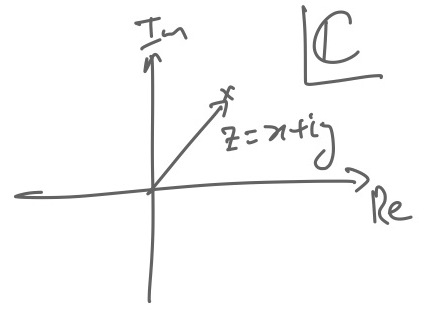
\includegraphics{figs/comp_argand}
  \caption{Argand diagram.}
\end{marginfigure}

Given $z=x+\zi y$, the \Def{conjugate} of $z$ is defined to be
$\zbar=x-\zi y$. Geometrically, this represents a reflection of $z$ in the
`real' axis. The \Def{real} and \Def{imaginary} part of $z$ is
given respectively by
\begin{equation*}
	\Real(z)=\frac{z+\zbar}{2},\qquad \Imag(z)=\frac{z-\zbar}{2}.
\end{equation*}

In polar form, $z=r(\cos\theta+\zi\sin\theta)$. $r$ is called the
\Def{modulus} of $z$ and is denoted $|z|$, whilst $\theta$ is called the
\Def{argument} of $z$, denoted $\mbox{arg}(z)$.

%-------------------------------------------------------------------------------

\section{Geometry of addition and multiplication in $\mathbb{C}$}

Addition is as in $\mathbb{R}^2$. From this, we can deduce the \Def{triangle
inequality}.
\begin{lemma}
	For $z_1,z_2\in\mathbb{C}$, $|z_1 +z_2|\leq|z_1|+|z_2|$, and we have an
	equality iff $\mbox{arg}(z_1)=\mbox{arg}(z_2)$. By corollary, we have $|z_2
	+z_2|\geq||z_1|-|z_2||$.
\end{lemma}
\begin{proof}
	Without loss of generalisation, let $|z_1|>|z_2|$, then $|z_1|=|z_1 + z_2 +
	(-z_2)|\leq|z_1+z_2|+|z_2|$ by the triangle inequality for real numbers. So
	$|z_1|-|z_2|\leq|z_1+z_2|$, and since $|z_1|>|z_2|$, we have the corollary
	of the result as required. \qed
\end{proof}

For multiplication, we observe that $|z_1 z_2|=|z_1||z_2|$ and $\mbox{arg}(z_1
z_2)=\mbox{arg}(z_1)+\mbox{arg}(z_2)$. Geometrically, this is a spiral scaling.

We can use the $\mathbb{C}$-plane to describe various geometrical objects.
\begin{example}
	A circle may be described by $|z-z_0|=a$, where $z_0$ is the centre of the
	circle and $a$ is the radius; expanding this accordingly, we see that $a^2 =
	(x-x_0)^2 + (y-y_0)^2$.
\end{example}
\begin{example}
	The equation $|z-x_0|+|z+x_0|=2r$ describes an ellipse, where $r>|x_0|$.
	This may be done via expansion in $(x,y)$. Alternatively, in polar form, we
	observe that, for $z=a+\zi b$, $|z\pm x_0|^2 = (a^2-b^2)\cos^2\theta\pm
	2ax_0\cos\theta + (x_0^2+b^2)$. If $x_0^2=(a^2-b^2)$, then this may be
	simplified to $|z\pm x_0|=a\pm x_0\cos\theta$ since $a>x_0$. With this, we
	obtain $|z-x_0|+|z+x_0|=2a$, thus, with $x=a\cos\theta$ and $y=b\sin\theta$,
	this describes an ellipse.
\end{example}
\begin{example}
	The locus of $|z-z_1|=|z-z_2|$ describes the line that is equidistant to the
	points $z_1$ and $z_2$. To see this, expanding everything in $x$ and $y$ and
	we obtain the equality
	\begin{equation*}
		x(x_2-x_1) + y(y_2-y_1) 
		= \frac{y_2^2-y_1^2}{2} + \frac{x_2^2 - x_1^2}{2},
	\end{equation*}
	and the normal to the line is $z_2-z_1$.
\end{example}

%-------------------------------------------------------------------------------

\section{de Moivre's theorem}

\begin{theorem}[de Moivre's theorem]
	For all $n\in\mathbb{Z}^+$ and angle $\theta$, $\cos n\theta+\zi \sin
	n\theta = (\cos\theta+\zi\sin\theta)^n$.
\end{theorem}
\begin{proof}
	We do this by induction. The $n=1$ case is trivial, so, assuming it is true
	for $n$, then we observe that
	\begin{align*}
		\cos(n+1)\theta&+\zi\sin(n+1)\theta \\
		&=\cos n\theta\cos\theta + \zi^2 \sin\theta\sin n\theta
		+\zi\sin n\theta\cos\theta + \zi\sin\theta\cos n\theta\\
		&= (\cos n\theta+\zi\sin n\theta)(\cos\theta+\zi\sin\theta)\\
		&=(\cos\theta+\zi\sin\theta)^{n+1}.
	\end{align*}
	\qed
\end{proof}

\begin{example}
  Since  
	\begin{equation*}
		\cos2\theta+\zi\sin2\theta=(\cos\theta+\zi\sin\theta)^2
		=(\cos^2\theta-\sin^2\theta)+\zi(2\sin\theta\cos\theta),
	\end{equation*}
	and remembering the double angle formulae, the equality agrees. From de
	Moivre's theorem, we see that
	\begin{equation*}
		\cos n\theta=\Real(\cos\theta+\zi\sin\theta)^n,\qquad
		\sin n\theta=\Imag(\cos\theta+\zi\sin\theta)^n.
	\end{equation*}
\end{example}

We can also use the theorem to find $\sin$ or $\cos$ of rational multiples of
$\pi$.
\begin{example}
	Express $\sin4\theta/\cos\theta$ as a polynomial in $\sin\theta$, and hence
	find $\sin(\pi/4)$.
	\begin{align*}
		\sin4\theta = \Imag(\cos\theta+\zi\sin\theta)^4
		&= 4\cos^3\theta\sin\theta-4\cos\theta\sin^3\theta\\
		&= 4\cos\theta(\sin\theta-2\sin^3\theta),
	\end{align*}
	so $\sin4\theta/\cos\theta=4\sin\theta(1-2\sin^\theta)$. Evaluating this
	$\pi/4$, we see that the LHS is zero. Now, $4\sin(\pi/4)>0$, so we conclude
	that $\sin(\pi/4)=1/\sqrt{2}$, as expected.
\end{example}
\begin{example}
	Find $\cos(k\pi/6)$ for $k=1,2,3,4,5$.\\
	
	Letting $c=\cos\theta$ and $s=\sin\theta$, observe that
	\begin{equation*}
		\sin6\theta=sc(6c^4+6s^4-20s^2c^2)=sc(32c^4-32c^2+6)
		=2sc(4c^3-3)(4c^2-1).
	\end{equation*}
	Now, $\sin(k\pi)=0$, so LHS is zero, and since $\sin(k\pi/6)\neq0$, we have
	\begin{equation*}
		\cos^2(k\pi/6)=3/4,\quad \cos^2(k\pi/6)=1/4,\quad \cos\theta=0,
	\end{equation*}
	which implies that
	\begin{equation*}
	  \cos(k\pi/6)=\pm\sqrt{3}/2,\ \pm1/2,\ 0.
	\end{equation*}
	Since $\cos\theta$ is a decreasing function in $[0,\pi]$, we have
	\begin{align*}
		\cos(\pi/6)=\sqrt{3}/2,\quad \cos(2\pi/6)=1/2,\quad \cos(\pi/2)=0,\\
		\cos(2\pi/3)=-1/2,\quad \cos(5\pi/6)=-\sqrt{3}/2.
	\end{align*}
\end{example}

%-------------------------------------------------------------------------------

\section{Imaginary exponentials}

de Moivre's theorem hints at a deeper geometric significance of cosine and sine
functions and a way of encoding multiplication by imaginary numbers. Suppose
$f(\theta)=\cos\theta+\zi\sin\theta$, then we notice that $f'(\theta)=\zi
f(\theta)$, and, more generally, $f^{(n)}(\theta)=\zi^n f(\theta)$. We know that
also that the $n$-th derivative of $\ex^{\lambda x}$ is $\lambda^n\ex^{\lambda
x}$, so this suggests a link with exponential functions; indeed, we have
\Def{Euler's formula}
\begin{equation}
	\cos\theta+\zi\sin\theta=\ex^{\zi\theta}.
\end{equation}
By de Moivre's theroem then,
\begin{equation*}
	r(\cos n\theta+\zi\sin n\theta)=r(\cos\theta+\zi\sin\theta)^n
	=r\ex^{\zi n\theta}.
\end{equation*}
\begin{lemma}[Euler identity]
	$\ex^{\zi\pi}+1=0$. \qedwhite
\end{lemma}
\begin{example}
	Find all the roots of $z^6+4z^3+8=0$.\\
	
	Factorising the above gives $z^3=-2\pm2\zi$. So since $|z^3|=2\sqrt{2}$, we
	have $|z|=\sqrt{2}$. Now,
	\begin{equation*}
		\mbox{arg}(-2+2\zi)=\frac{3\pi}{4},\qquad
		\mbox{arg}(-2-2\zi)=\frac{5\pi/4},
	\end{equation*}
	and the argument of the roots $z$ satisfies
	\begin{equation*}
		\mbox{arg}(z)=\frac{3\pi/4 + 2n\pi}{3},\qquad
		\mbox{arg}(z)=\frac{5\pi/4 + 2n\pi}{3},
	\end{equation*}
	where the division by $3$ is to take into account the cube root, and the
	$2n\pi$ factors is to account for all the roots. This eventually yields
	\begin{equation*}
		z=\sqrt{2}(\ex^{\zi\pi/4}, \ex^{5\zi\pi/4}, \ex^{11\zi\pi/12},
		\ex^{13\zi\pi/12}, \ex^{19\zi\pi/12}, \ex^{21\zi\pi/21}).
	\end{equation*}
\end{example}

%===============================================================================

\chapter{Basics of complex functions}

A real function can for example be once differentiable, but not
twice. One example is $f(x) = x|x|$, where $f'(x)$ is not differentiable at
$x=0$.

\begin{theorem}
  If a complex function is once differentiable, it is differentiable as many
  times as you like.
\end{theorem}

It is possible for two real functions to agree on an interval but not
everywhere, assuming they are differentiable. One example is $f(x) = x|x|$ and
$g(x) = x^2$ for $x>0$.

\begin{theorem}
  If two complex differentiable functions agree on any disc in the complex
  plane, then they agree everywhere (subject to certain conditions...)
\end{theorem}

Recall that a real function assigns any real number $x$ to at most one real
number (i.e. it is injective). A \Def{complex function} therefore assigns any
complex number $z$ to at most one complex number. These include standard
polynomials, rational functions, transcendental functions, trigonometric
functions, hyperbolic functions, where the argument is in $z$. Some examples
have already been given above.

\begin{example}
  Solve $\ex^z = 1$.\\
  
  Writing $z = x + \zi y$ and using Euler's formula,
  \begin{equation*}
    \ex^x (\cos y + \zi \sin y) = 1,
  \end{equation*}
  and equating real and imaginary parts lead to
  \begin{equation*}
    \ex^x \cos y = 1, \qquad \ex^x \sin y = 0.
  \end{equation*}
  Considering the imaginary part, since $\ex^x \neq 0$, $y = n\pi$ for $n \in
  \mathbb{Z}$, but from the real part, since $\ex^x > 0$ and $\cos n\pi = \pm
  1$, we should only have $y = 2n\pi$ for $n \in \mathbb{Z}$. The real part then
  additionally implies that $x=0$ since $\cos 2n\pi = 1$, so $z = 2\zi n \pi$
  for $n \in \mathbb{Z}$.
\end{example}
Note that $|\ex^{\zi z}| \geq 0$ for all $z \in \mathbb{C}$.

\begin{example}
  Solve $\sin z = 0$.\\
  
  With the standard identity for sine with complex arguments, we have
  \begin{equation*}
    \frac{\ex^{\zi z} - \ex^{-\zi z}}{2\zi} = 0.
  \end{equation*}
  Equating real and imaginary parts lead to $z = m\pi$, $m \in \mathbb{Z}$.
\end{example}

The (natural) \Def{logarithm} we define by
\begin{equation}
  \log z = \log|z| + \zi \mbox{arg}z
\end{equation}
to give a complex version of the log function that satisfies the usual rules of
\begin{equation*}
  \log z = \log r\ex^{\zi\theta} = \log r + \zi \theta = \log|z| + \zi \mbox{arg}z.
\end{equation*}
Here we need to choose a \Def{branch}, and we take $\theta\in(-\pi, \pi)$ (the
\Def{principal branch}) to preserve the continuity property, so that $\log z$ is
undefined on the negative real axis, coinciding with the real case.

\begin{example}
  $\log(1-i) = \log\sqrt{2} - \zi(\pi / 4)$
\end{example}

We use $\log z$ to define powers of complex numbers. Recall that for real
numbers we have $x^a = \ex^{a \log a}$ for $a>0$, so for $z,w \in \mathbb{C}$,
we analogously define 
\begin{equation}
  z^w = \ex^{w \log z},
\end{equation}
choosing the principal branch unless otherwise stated.

\begin{example}
  \begin{align*}
    (1 + \zi \sqrt{3})^{1/2} &= \exp\left[\frac{1}{2} \log(1 + \zi \sqrt{3})\right] \\
    &= \exp\left[\frac{1}{2} \left(\log 2 + \zi\frac{\pi}{3}\right)\right] \\
    &= \ex^{\log \sqrt{2}} \ex^{\zi(\pi/6)} \\
    &= \sqrt{2}\ex^{\zi(\pi/6)},
  \end{align*}
  which in this case is could have been gotten from $(1 + \zi \sqrt{3}) = 2\ex^{\zi(\pi/3)}$.
\end{example}

\begin{example}
  \begin{align*}
    (1 - \zi)^{\zi} = \ex^{\zi \log(1-\zi)} = \ex^{\zi (\log \sqrt{2} - \zi \pi/4)} = \ex^{\pi/4} \ex^{\zi \log\sqrt{2}}.
  \end{align*}
\end{example}

We say a complex function $f(z)$ is \Def{complex differentiable at $z = z_0$} if
\begin{equation*}
  \lim_{z\to z_0} \frac{f(z) - f(z_0)}{z - z_0}
\end{equation*}
exists, or that
\begin{equation*}
  \lim_{h\to 0} \frac{f(z + h) - f(z)}{h}
\end{equation*}
exists at $z = z_0$. The derivative is denoted $f'(z)$ as usual.

\begin{example}
  For $f(z) = z^2$,
  \begin{equation*}
    \lim_{h \to 0} \frac{f(z + h) - f(z)}{h} = \lim_{h \to 0} \frac{z^2 + 2hz + h^2 - z^2}{h} = \lim_{h \to 0} 2z + h = 2z.
  \end{equation*}
  $f(z)$ is differentiable everywhere.
\end{example}
The usual rules for differentiation hold (linearity, product rule, chain rule
etc.)

Note that $f(x) = x|x|$ is real differentiable everywhere. $f(z) = z|z|$ on the
other hand is differentiable on the real axis, and complex differentiable at the
origin.

Complex differentiation is a much stronger condition. Recall that for the limit
to exist in the real case, the limit only needs to be equal when approached from
above or below on the real line. In the complex plane however there are an
infinite numbers of cases the limit can be approach, and thus a infinite number
of cases to check. We see that a necessary condition for complex
differentiability is that the limit needs to exist when $z_0$ is approached in
the lines parallel to the real and imaginary axis. If we set $f(z)$ to be
\begin{equation*}
  f(z) = u(x,y) + \zi v(x,y)
\end{equation*}
for some real functions $u$ and $v$, then it turns out that
\begin{align*}
  \lim_{z \to z_0} \frac{f(z) - f(z_0)}{z - z_0} = \ddy{u}{x} + \zi \ddy{v}{x} = \ddy{v}{y} - \zi \ddy{u}{y},
\end{align*}
when we take the limit in the direction parallel to the real and imaginary axis
respectively. It follows that a \emph{necessary} conditions for a function to be
complex differentiable is that
\begin{equation}
  \ddy{u}{x} = \ddy{v}{y} \qquad \textnormal{and} \qquad \ddy{u}{y} = -\ddy{v}{x}.
\end{equation}
These are known as the \Def{Cauchy--Riemann equations}, and we actually have the
following theorem.
\begin{theorem}
  If $f(z)$ is complex differentiable at $z = z_0$, then the Cauchy--Riemann
  equations hold at $(x_0, y_0)$ for $z_0 = x_0 + \zi y_0$, and that
  \begin{equation*}
    f'(z_0) = \left.\left(\ddy{u}{x} + \zi \ddy{v}{x}\right)\right|_{(x_0, y_0)} = \left.\left(\ddy{v}{y} - \zi \ddy{u}{y}\right)\right|_{(x_0, y_0)}.
  \end{equation*}
\end{theorem}
\begin{proof}
  If we approach $z_0$ in a line parallel to the real axis, we have
  \begin{align*}
    f'(z_0) 
      &= \lim_{x \to x_0} \frac{u(x, y_0) + \zi v(x, y_0) - u(x_0, y_0) - \zi v(x_0, y_0)}{x - x_0}\\
      &= \lim_{x \to x_0} \left(\frac{u(x, y_0) - u(x_0, y_0)}{x - x_0} + \zi \frac{v(x, y_0) - v(x_0, y_0)}{x - x_0}\right)\\
      &= \left.\ddy{u}{x}\right|_{(x_0, y_0)} + \zi \left.\ddy{v}{x}\right|_{(x_0, y_0)}.
  \end{align*}
  We have the analogous result when approaching $z_0$ in a line parallel to the
  imaginary axis. \qed
\end{proof}

In actual fact, the Cauchy--Riemann equation holding is a necessary \emph{and}
sufficient condition for complex differentiability.

\begin{theorem}
  Let $f(z) = u(x,y) + \zi v(x,y)$. If the partial derivatives of $u$ and $v$
  exist in some disk centered on $(x_0, y_0)$ and are continuous at $z_0 = x_0 +
  \zi y_0$, and $u$ and $v$ satisfy the Cauchy--Riemann equation, then $f(z)$ is
  complex differentiable at $z_0$. \qedwhite
\end{theorem}

A function is said to be \Def{holomorphic} (or \Def{analytic}) at $z_0$ if it is
complex differentiable on some disk centred at $z_0$. A function is holomorphic
if it is analytic at all points where it is defined.

\begin{example}
  If $f(z) = y^3 - 3\zi x y^2$, fine where $f(z)$ is complex differentiable, and
  compute $f'(z)$.\\
  
  Note that for $u = y^3$ and $v = -3xy^2$,
  \begin{equation*}
    \ddy{u}{x} = 0, \quad \ddy{v}{x} = -3y^2, \quad \ddy{u}{y} = -3y^2, \quad \ddy{v}{y} = -6xy,
  \end{equation*}
  so it is differentiable if $-6xy = 0$ and $3y^2 = 3y^2$, which is only
  satisfied at $x=0$ or $y=0$, i.e. at the co-ordinate axes. In this case $f'(z)
  = -\zi 3y^2$, and that $f(z)$ is nowhere holomorphic.
\end{example}

\begin{theorem}
  Let $f(z)$ be holomorphic and $f(z) = u(x,y) + \zi v(x,y)$. Then $u$ and $v$
  are solutions to Laplace's equation in two dimensions.
\end{theorem}
\begin{proof}
  By Cauchy--Riemann equations and the holomorphic property,
  \begin{equation*}
    \ddy{^2 y}{x^2} = \ddy{}{x}\ddy{u}{x} = \ddy{v}{x\partial y} = \ddy{v}{y\partial x} = \ddy{}{y}\ddy{v}{x} = \ddy{}{y}\left(-\ddy{u}{y}\right) = -\ddy{^2 u}{y^2},
  \end{equation*}
  so that $\partial^2 u / \partial x^2 + \partial^2 u / \partial y^2 = 0$.
  Similarly for $v$. \qed
\end{proof}

Recall that if $f(x)$ is an infinitely differentiable real function, that its
Taylor series about $x = x_0$ is given by
\begin{equation*}
  \sum^\infty_{k=0} \frac{f^{(k)}(x_0)}{k!}(x - x_0)^k.
\end{equation*}
The complex counterpart is then if $f(z)$ is an infinitely complex
differentiable complex function, its Taylor series about $z = z_0$ is
\begin{equation*}
  \sum^\infty_{k=0} \frac{f^{(k)}(z_0)}{k!}(z - z_0)^k.
\end{equation*}
Since derivatives of standard functions are the same in the complex case, their
Taylor series are the same too.

\begin{theorem}
  Let $f(z)$ be complex differentiable. Then its Taylor series converges to
  $f(z)$ for all $z$ where it converges. \qedwhite
\end{theorem}
This implies any complex differentiable function is just a power series.

If we let $\sum^\infty_{n=0} b_n (z - z_0)^n$ be a power series centred on $z =
z_0$, then there exists some $R \in [0, \infty]$ where the power series
\begin{itemize}
  \item converges for $|z - z_0| < R$,
  \item diverges for $|z - z_0| > R$,
  \item inconclusive for $|z - z_0| = R$.
\end{itemize}
$R$ is called the \Def{radius of convergence}, and $\{z : |z - z_0| < R\}$ is
the \Def{disk of convergence}.

To find the disk of convergence we can often use the ratio test.

\begin{example}
  Find the radius of convergence for $f(z) = (1 - z)^{-1}$ around $z_0 = 0$.\\
  
  Recall that $f(z) = \sim^\infty_{n=0} z^n$, then we note that $\lim_{n \to
  \infty} |z^{n+1} / z^n| = |z|$, hence we have convergence if $|z| < 1$ by the
  ratio test, and the radius of convergence is $R = 1$.
\end{example}

\begin{example}
  For $f(z) = \sum^\infty_{n=0} n^2 (z - \zi)^{2n} / 2^n$ as a power series around
  $z_0 = \zi$, by the ratio test,
  \begin{equation*}
    \lim_{n \to \infty} \left|\frac{(n+1)^2 (z - \zi)^{2n+2}}{2^{n+1}}\frac{2^n}{n^2 (z-\zi)^{2n}}\right| = \frac{|z - \zi|^2}{2},
  \end{equation*}
  so we have convergence if $|z - \zi| < \sqrt{2}$, and the radius of
  convergence is $R = \sqrt{2}$.
\end{example}

\begin{theorem}
  If $\sum^\infty_{n=0} a_n (z - z_0)^n$ has radius of convergence $R$ and
  converges to $f(z)$ of its disk of convergence $D$, then $f(z)$ is complex
  differentiable, and $\sum^\infty_{n=0} a_n n (z - z_0)^{n-1}$ converges to
  $f'(z)$ in $D$. \qedwhite
\end{theorem}

\begin{theorem}
  If $\sum^\infty_{n=0} a_n (z - z_0)^n \to f(z)$ in its disk of convergence,
  then $f(z)$ is complex differentiable an infinite number of times, and
  $f^{(n)}(z_0) = n! a_n$.
\end{theorem}
\begin{proof}
  By previous theorem, we have
  \begin{align*}
    f(z)   &= a_0 + a_1 (z - z_0) +   a_2 (z - z_0)^2 + \ldots\\
    f'(z)  &=       a_1           + 2 a_2 (z - z_0)   + \ldots\\
    f''(z) &=                       2\cdot 1 a_2      + \ldots
  \end{align*}
  and so on. Hence the function is infinitely complex differentiable, and
  $f^{(n)}(z_0)$ is as required. \qed
\end{proof}

\begin{example}
  Find the Taylor series of $(1 - z)^{-2}$ about $z = 0$.\\
  
  We see that since $\mathrm{d}/\mathrm{d}z (1 - z)^{-1} = (1 - z)^{-2}$,
  \begin{equation*}
    \frac{1}{(1 - z)^2} = \sum^\infty_{n=1} n z^{n-1}, \qquad |z| < 1.
  \end{equation*}
\end{example}

\begin{example}
  Find the Taylor series for $\cosh(4z^3)$ about $z = 0$.\\
  
  Recall that
  \begin{equation*}
    \cosh y = 1 + \frac{y^2}{2!} + \ldots = \sum^\infty_{n=0} \frac{y^{2n}}{(2n)!},
  \end{equation*}
  so that
  \begin{equation*}
    \cosh(4z^3) = \sum^\infty_{n=0} \frac{(4z^3)^{2n}}{(2n)!} = \sum^\infty_{n=0} \frac{16^n z^{6n}}{(2n)!}, \qquad \forall z \in \mathbb{C}.
  \end{equation*}
\end{example}

\begin{example}
  Find the Taylor series of $z^3 / (1-5z)^2$ about $z = 0$.\\
  
  Using the identity from two examples ago,
  \begin{equation*}
    \frac{1}{(1-5z)^2} = \sum^\infty_{n=1} n (5z)^{n-1},
  \end{equation*}
  so that
  \begin{equation*}
    \frac{z^3}{(1-5z)^2} = \sum^\infty_{n=1} n 5^{n-1} z^{n+2}, \qquad |z| < \frac{1}{5}.
  \end{equation*}
\end{example}

\begin{example}
  Find the Taylor series for $3z(z+1)^{-1}(z-2)^{-1}$ about $z = 0$.\\
  
  First note that the radius of convergence cannot be greater than 1. By partial
  fractions,
  \begin{equation*}
    \frac{3z}{(z+1)(z-2)} = \frac{1}{z+1} + \frac{2}{z-2},
  \end{equation*}
  so that the Taylor series is
  \begin{equation*}
    \sum^\infty_{n=0} (-z)^n - \sum^\infty_{n=0} \left(\frac{z}{2}\right)^n = \sum^\infty_{n=0} \left[(-1)^n - \frac{1}{2^n}\right] z^n, \qquad |z| < 1.
  \end{equation*}
\end{example}

%===============================================================================

\chapter{Integration in the complex plane}

Recall that in the real case we have the \Def{indefinite integral} with
\begin{equation*}
  \int f(x)\; \mathrm{d}x = F(x),
\end{equation*}
where $F(x)$ is the primitive of $f$. We also have the \Def{definite integral}
where, by the fundamental theorem of calculus, gives
\begin{equation*}
  \int^a_b f(x)\; \mathrm{d}x = F(b) - F(a).
\end{equation*}
Although we can generalise the indefinite integral to the complex case, the
definite integral doesn't generalise directly, because we are essentially trying
to talk about a 2-dimensional surface in 4-space. So instead we integrate
complex functions along curves, or contours, in the complex plane.

%-------------------------------------------------------------------------------

\section{Curves in $\mathbb{C}$}

A differentiable curve in $\mathbb{C}$ is a function $\gamma : [a, b] \to
\mathbb{C}$ such that $\gamma(t) = \gamma_1(t) + \zi \gamma_2 (t)$, where
$\gamma_1$ and $\gamma_2$ are real differentiable functions in $t$.

\begin{example}
  One way to generate the unit circle is with
  \begin{equation*}
    \gamma : [0, 1] \to \mathbb{C}, \qquad \gamma(t) = \ex^{2\pi \zi t}.
  \end{equation*}
  \begin{marginfigure}
    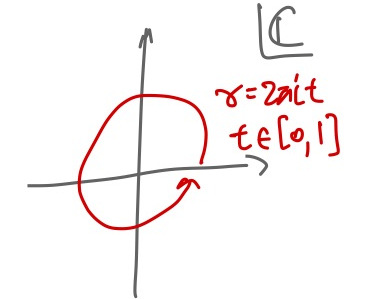
\includegraphics{comp_unit_circle}
    \caption{Unit circle transversed in the positive sense.}
  \end{marginfigure}
  Notice here that $\gamma$ is closed, and has a direction characterised by how
  $t$ is parameterised (in this case it is in the positive sense, or in the
  anti-clockwise). In general, a circle centred at $z_0$ with radius $r$ has the
  associated curve
  \begin{equation*}
    \gamma : [0, 1] \to \mathbb{C}, \qquad \gamma(t) = z_0 + r \ex^{2\pi \zi t}.
  \end{equation*}
\end{example}

\begin{example}
  \begin{marginfigure}
    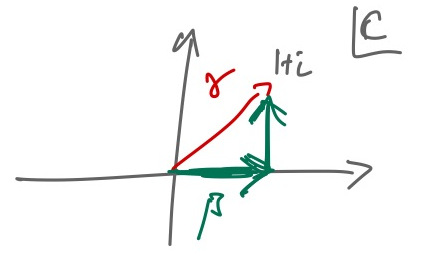
\includegraphics{comp_split_curve}
    \caption{Two paths getting to the same point.}
  \end{marginfigure}
  Consider two curves
  \begin{equation*}
    \gamma(t) = t + \zi t, \quad 0 \leq t \leq 1, \qquad \beta(t) = \begin{cases}t, & 0 \leq t \leq 1, \\ 1 + (t-1)\zi & 1 \leq t \leq 2. \end{cases}
  \end{equation*}
  
  Both curves connect the origin to $z = 1 + \zi$, but the path is different.
  $\beta(t)$ here is piecewise differentiable. One question of course is whether
  the path matters (see later). In general, a vector from $z_0$ to $z_1$ may be
  parameterised as $\gamma(t) = z_0 + t (z_1 - z_0)$, for $t \in [0, 1]$.
\end{example}

%-------------------------------------------------------------------------------

\subsection{Contour integrals}

To integrate along the curve $z = \gamma(t)$ with $t\in[a, b]$, we have from
chain rule that $\mathrm{d}z = \gamma'(t)\; \mathrm{d}t$, so that
\begin{equation*}
  \int_{\gamma} f(z)\; \mathrm{d}z = \int^b_a f(\gamma(t)) \gamma'(t)\; \mathrm{d}t,
\end{equation*}
where the latter is as before since we are dealing with a function of a real
variable.

\begin{example}
  Compute the contour integrals of the following:
  \begin{enumerate}
    \item $f(z) = z^2$, $\gamma(t) = \ex^{\zi \pi t}$, $t \in [0, 1]$\\
    
    \begin{marginfigure}
      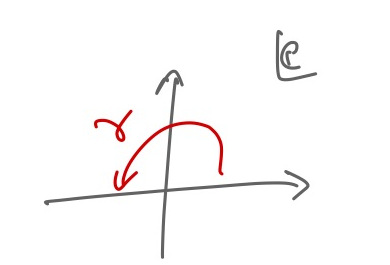
\includegraphics{figs/comp_upper_semicircle}
      \caption{Upper semi-circle transversed in the positive sense.}
    \end{marginfigure}
    
    The path is the upper unit semi-circle, and we have
    \begin{equation*}
      \int_\gamma f(z)\; \mathrm{d}z = \zi \pi \int^1_0 \ex^{3\zi\pi t}\; \mathrm{d}t = -\frac{2}{3}.
    \end{equation*}
    
    \item $f(z) = z^2$, $\gamma(t) = \ex^{-\zi \pi t}$, $t \in [0, 1]$\\
    
    \begin{marginfigure}
      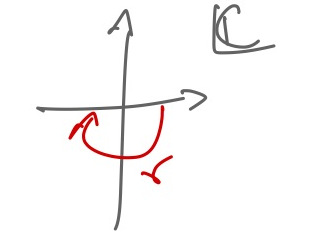
\includegraphics{figs/comp_lower_semicircle}
      \caption{Lower semi-circle transversed in the \emph{negative} sense.}
    \end{marginfigure}
    
    The path is the lower unit semi-circle, and we have
    \begin{equation*}
      \int_\gamma f(z)\; \mathrm{d}z = -\zi \pi \int^1_0 \ex^{-3\zi\pi t}\; \mathrm{d}t = -\frac{2}{3}.
    \end{equation*}
    
    Notice here the integral has the same value as the previous part, which in
    this case is not a coincidence.
    
    \item $f(z) = \overline{z}$, $\gamma(t) = 1 + \zi t$, $t \in [0, 2]$\\
    
    We have
    \begin{equation*}
      \int_\gamma f(z)\; \mathrm{d}z = \zi \int^2_0 (1 - \zi t)\; \mathrm{d}t = 2 + 2\zi.
    \end{equation*}
  \end{enumerate}
\end{example}

A \Def{contour} is a continuous curve made up a finite number of differentiable
curves. The contour itself does not need to be differentiable although the
individual pieces should. The integral of $f(z)$ along a contour is then the sum
of integrals along each individual differentiable curve.

\begin{proposition}
  We have the following properties for contour integrals:
  \begin{enumerate}
    \item Linearity, where
    \begin{equation*}
      \int_\gamma (\alpha f(z) + \beta g(z))\; \mathrm{d}z = \alpha \int_\gamma f(z)\; \mathrm{d}z + \beta \int_\gamma g(z))\; \mathrm{d}z.
    \end{equation*}
    
    \item If contours $\gamma_1$ and $\gamma_2$ have the same track in
    $\mathbb{C}$ and transverse it in the same direction, then
    \begin{equation*}
      \int_{\gamma_1} f(z)\; \mathrm{d}z = \int_{\gamma_2} f(z)\; \mathrm{d}z.
    \end{equation*}
    
    \item If $\gamma : [a,b] \to \mathbb{C}$ and $\mu : [-b, -a] \to \mathbb{C}$
    where $\mu(t) = \gamma(-t)$, i.e. $\mu$ is the `reverse' of $\gamma$, then
    \begin{equation*}
      \int_{\mu} f(z)\; \mathrm{d}z = -\int_{\gamma} f(z)\; \mathrm{d}z.
    \end{equation*}
    
    \item We have the inequality
    \begin{equation*}
      \left|\int_\gamma f(z)\; \mathrm{d}z\right| \leq \int_\gamma |f(\gamma(t))| \cdot |\gamma'(t)|\; \mathrm{d}t \leq \textnormal{length}(\gamma) \cdot \max_{\gamma} |f(\gamma(t))|.
    \end{equation*}
    
    \item (Fundamental Theorem of Calculus) Let $F(z)$ be holomorphic on an open
    set $D \subset \mathbb{C}$, and $F'(z) = f(z)$. Then for any contour $\gamma
    : [a,b] \to D$ with end points $z_0 = \gamma(a)$ and $z_1 = \gamma(b)$, we
    have
    \begin{equation*}
      \int_\gamma f(z)\; \mathrm{d}z = F(z_1) - F(z_0).
    \end{equation*}
  \end{enumerate}
\end{proposition}

\begin{proof}
  \begin{enumerate}
    \item Since we have linearity when the integrals are real, this one is just
    by definition:
    \begin{align*}
      \int_\gamma (\alpha f(z) + \beta g(z))\; \mathrm{d}z 
        &= \int^b_a [\alpha f(\gamma(t)) + \beta g(\gamma(t))]\gamma'(t)\; \mathrm{d}t\\
        &= \alpha \int^b_a f(\gamma(t)) \gamma'(t)\; \mathrm{d}t + \beta \int^b_a g(\gamma(t)) \gamma'(t)\; \mathrm{d}t\\
        & =\alpha \int_\gamma f(z)\; \mathrm{d}z + \beta \int_\gamma g(z))\; \mathrm{d}z.
    \end{align*}
    
    \item Let $\gamma_k : [a_k, b_k] \to \mathbb{C}$ with $k=1,2$, and assume
    that $\gamma_2(h(t)) = \gamma_1(t)$. Then taking a substitution $u = h(t)$
    and judicious use of chain rule gives
    \begin{align*}
      \int_{\gamma_2} f(z)\; \mathrm{d}z &= \int^{b_2}_{a_2} f(\gamma_2(u)) \gamma_2'(u)\; \mathrm{d}u \\
      &= \int^{b_1}_{a_1} f(\gamma_2(h(t))) \gamma_2'(h(t)) h'(t)\; \mathrm{d}t \\
      &= \int^{b_1}_{a_1} f(\gamma_1(t)) \gamma_1'(t)\; \mathrm{d}t \\
      &= \int_{\gamma_1} f(z)\; \mathrm{d}z.
    \end{align*}
    
    \item As in previous case but use different limits.
    
    \item Let $\theta = \mbox{arg} \int_\gamma f(z)\; \mathrm{d}z$, then
    \begin{align*}
      \left|\int_\gamma f(z)\; \mathrm{d}z\right| &= \ex^{-\zi \theta} \int_\gamma f(z)\; \mathrm{d}z \\
      &= \int_\gamma \ex^{-\zi \theta} f(z)\; \mathrm{d}z \\
      &= \mbox{Re} \left(\int_\gamma \ex^{-\zi \theta} f(z)\; \mathrm{d}z\right) \\
      &= \mbox{Re} \left(\int^b_a \ex^{-\zi \theta} f(\gamma(t)) \gamma'(t)\; \mathrm{d}t\right)\\
      &\leq \int^b_a \left|\ex^{-\zi \theta} f(\gamma(t)) \gamma'(t)\right|\; \mathrm{d}t \\
      &= \int^b_a |f(\gamma(t))| \cdot |\gamma'(t)|\; \mathrm{d}t\\
      &\leq \textnormal{length}(\gamma) \cdot \max_{\gamma} |f(\gamma(t))|.
    \end{align*}
    
    \item Let $F(\gamma(t)) = u(t) + \zi v(t)$, where $u$ and $v$ are real
    functions. By the chain rule, $u'(t) + \zi v'(t) = F'(\gamma(t))\gamma'(t)$,
    so
    \begin{align*}
      \int_\gamma f(z)\; \mathrm{d}z = \int^b_a F'(\gamma(t))\gamma'(t)\; \mathrm{d}t = \int^b_a [u'(t) + \zi v'(t)]\; \mathrm{d}t = F(b) - F(a).
    \end{align*}
  \end{enumerate}
\end{proof}

\begin{example}
  Let $\gamma(t) = R\ex^{\zi t}$, $t\in[0, 2\pi]$, then
  \begin{equation*}
    \int_\gamma \frac{1}{z}\; \mathrm{d}z = \int^{2\pi}_0 \frac{1}{R\ex^{\zi t}} R\zi \ex^{\zi t}\; \mathrm{d}t = 2\pi \zi,
  \end{equation*}
  and this is because the primitive is not well-defined at $z=0$.
\end{example}

\begin{theorem}[Path Independent Theorem]
  Let $f$ be continuous on an open connected set $D \subset \mathbb{C}$. Then
  the following statements are equivalent to each other:
  \begin{enumerate}
    \item integrals are path independent;
    \item if $\gamma$ is a closed curve in $D$, then $\oint_\gamma f(z)\; \mathrm{d}z = 0$;
    \item there exists a primitive $F(z)$ of $f(z)$ where $F'(z) = f(z)$,
    defined globally on $D$.
  \end{enumerate}
\end{theorem}

\begin{proof}
  We show that 1 is equivalent to 2, and 2 is equivalent to 3, so 1 is then
  equivalent to 3 by default.
  
  (1 $\Leftrightarrow$ 2) Suppose $\Gamma$ is a closed curve consisting of some
  arbitrary closed simple curves $\gamma_{0,1}$ as illustrated.
  \begin{marginfigure}
    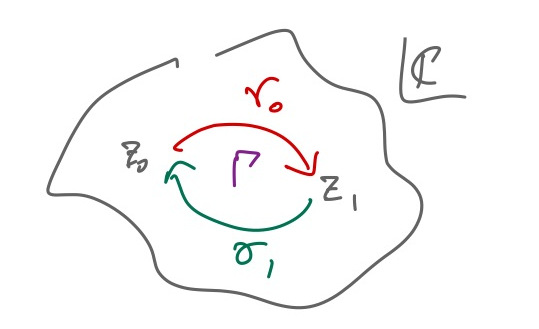
\includegraphics{comp_joined_curve}
    \caption{A joined path.}
  \end{marginfigure}
  
  Then
  \begin{equation*}
    \oint_\Gamma f(z)\; \mathrm{d}z = \left(\int_{\gamma_0} + \int_{-\gamma_1}\right) f(z)\; \mathrm{d}z = \left(\int_{\gamma_0} - \int_{\gamma_1}\right) f(z)\; \mathrm{d}z.
  \end{equation*}
  Since the integrals are path independent, we have $\int_{\Gamma} f(z)\;
  \mathrm{d}z = 0$. Conversely, if the integral is zero by assumption, since
  $\gamma_{0,1}$ are arbitrary, this implies path independence.
  
  (2 $\Leftrightarrow$ 3) Assuming there is a primitive, then the fundamental
  theorem of calculus implies that since we have the existence of the primitive,
  we have $\int_\gamma f(z)\; \mathrm{d}z = F(z_1) - F(z_0)$ regardless of path,
  so if $z_1 = z_0$ then $\oint_\gamma f(z)\; \mathrm{d}z = 0$.
  
  Conversely, let $z_0$ be any fixed point on $D$, and $z$ be any other point on
  $D$. Since $D$ is open and connected, the contour $\gamma$ joining $z_0$ to
  $z$ exists. Defining then $F(z) = \int_\gamma f(\zeta)\; \mathrm{d}\zeta$, by
  the assumption of of path independence, $F(z)$ is well-defined, and by the
  estimation property, $F'(z) = f(z)$, so there exists a primitive. \qed
\end{proof}

%-------------------------------------------------------------------------------

\subsection{Cauchy's theorem and corollaries}

Cauchy's theorem is one of the centre pieces of complex analysis. Before the
statement, we need an extra tool from topology regarding simple closed curves.

\begin{theorem}[Jordan curve theorem]
  Let $\gamma$ be a simple closed contour, i.e. no self-intersections except at
  the end points. Then the compliment of $\gamma$ in $\mathbb{C}$ is the
  disjoint union of exactly two sets, where exactly one is bounded. \qedwhite
\end{theorem}

Intuitively this says that a simple closed curve splits the space into an
outside and inside (trivial as it may sound rigourously proofing this is not so
obvious...)

\begin{theorem}[Cauchy's theorem]
  Let $f(z)$ be holomorphic on and inside a simple closed curve $\gamma$. Then
  $\oint_\gamma f(z)\; \mathrm{d}z = 0$.
\end{theorem}

\begin{proof}
  Let $f = u + \zi v$ for real $u$ and $v$, then using Green's theorem (since
  the resulting integrands are real)
  \begin{align*}
    \oint_\gamma f(z)\; \mathrm{d}z &= \oint_\gamma (u + \zi v)(\mathrm{d}x + \zi \mathrm{d}y) \\
      &= \oint_\gamma \left[(u\; \mathrm{d}x - v\; \mathrm{d}y) + \zi(u\; \mathrm{d}y + v\; \mathrm{d}x) \right]\\
      &= \iint_A \left[\left(-\ddy{u}{y} -\ddy{v}{x}\right) + \zi \left(\ddy{u}{x} - \ddy{v}{y}\right)\right] = 0.
  \end{align*}
  The latter quality to zero is because $f(z)$ is holomorphic, so $u$ and $v$
  satisfies the Cauchy--Riemann equations, and thus the partials are continuous
  and equal. \qed
\end{proof}

\begin{example}
By Cauchy's theorem, $\oint_{|z| = 1} z^n\; \mathrm{d}z = 0$ for all $n \geq 0$.
On the other hand, Cauchy's theorem doesn't tell us anything if $n < 0$ because
$f(z)$ is then not holomorphic at $z=0$. However, the above integral is zero for
all $n \neq -1$ by the fundamental theorem of calculus since a primitive exists
and is well-defined on the contour.

If $\gamma$ is some contour not enclosing $z = 0$, then $\oint_\gamma z^n\;
\mathrm{d}z = 0$ for all $n \geq 0$.
\end{example}

\begin{example}
  For $\oint_\gamma \exp[\cos z^3]\; \mathrm{d}z$, while we can't directly find
  a primitive of the integrand, since the integrand is a composite of
  holomorphic functions, the integrand is holomorhpic, and the integral is zero
  by Cauchy's theorem.
\end{example}

\begin{example}
  \begin{marginfigure}
    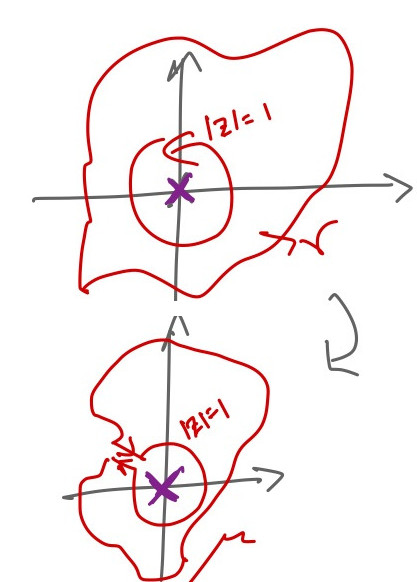
\includegraphics{comp_keyhole}
    \caption{A keyhole curve.}
  \end{marginfigure}
  It can be shown that if the curve $\gamma$ encloses $z=0$, then $\oint_\gamma
  z^{-1}\; \mathrm{d}z = 2\pi \zi$. Consider the curve as illustrated. If the gap
  between the `cut' is small enough, the line integrals going into the unit
  circle cancels each other, giving
  \begin{equation*}
    \oint_\mu \frac{1}{z}\; \mathrm{d}z = \oint_\gamma \frac{1}{z}\; \mathrm{d}z - \oint_{|z| = 1} \frac{1}{z}\; \mathrm{d}z.
  \end{equation*}
  By Cauchy's theorem, $\oint_\mu \frac{1}{z}\; \mathrm{d}z = 0$, so then
  \begin{equation*}
    \oint_\gamma \frac{1}{z}\; \mathrm{d}z = \oint_{|z| = 1} \frac{1}{z}\; \mathrm{d}z = 2\pi \zi.
  \end{equation*}
\end{example}

Note that Cauchy's theorem holding implies $\oint_\gamma f(z)\; \mathrm{d}z =
0$, which implies the primitive of $f(z)$ exists, and vice-versa. Although this
of course does not mean we can write the primitive down in closed form.

Consider how many times a contour $\gamma$ winds around a point $z_0$, as
illustrated. More formally, let $\gamma$ be a closed curve in $\mathbb{C}$ and
$z_0 \in \mathbb{C}$ be a point not on $\gamma$. The \Def{winding number} of
$\gamma$ with respect to $z_0$ is
\begin{equation}
  I(\gamma; z_0) = \frac{1}{2\pi\zi} \oint_\gamma \frac{\mathrm{d}z}{z - z_0}.
\end{equation}
\begin{marginfigure}
  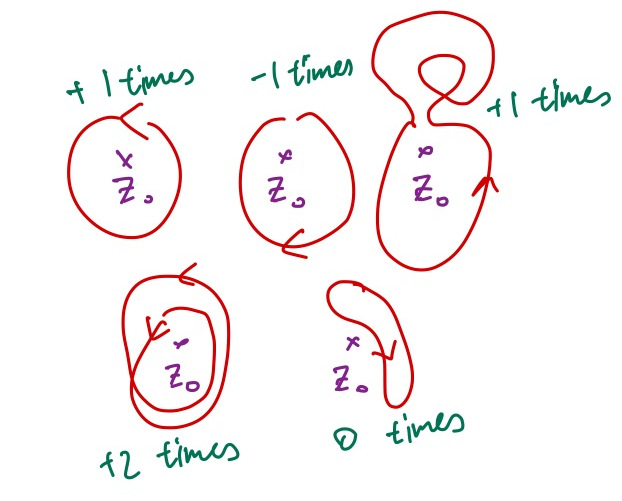
\includegraphics{figs/comp_winding_number}
  \caption{Illustrating the \textbf{winding number} of a curve around some
  point.}
\end{marginfigure}

\begin{theorem}
  Let $\gamma : [a,b]$ be a (piece-wise) closed curve and $z_0$ not on $\gamma$.
  Then $I(\gamma; z_0) \in \mathbb{Z}$.
\end{theorem}
\begin{proof}
  Consider.
  \begin{equation*}
    g(t) = \int_a^t \frac{\gamma'(s)}{\gamma(s) - z_0}\; \mathrm{d}s.
  \end{equation*}
  At points where the integrand is continuous, by the fundamental theorem of
  calculus, we have
  \begin{equation*}
    g'(t) = \frac{\gamma'(t)}{\gamma(t) - z_0} \quad \Rightarrow \quad \frac{\mathrm{d}}{\mathrm{d}t} \ex^{-g(t)}[\gamma(t) - z_0] = 0
  \end{equation*}
  for all $t$ such that $g'(t)$ exists. Since the time-derivative of the
  continuous function is zero, the function is constant and equal to
  $\ex^{-g(a)}[\gamma(a) - z_0]$. By a similar argument, we must have
  \begin{equation*}
    \ex^{-g(a)}[\gamma(a) - z_0] = \ex^{-g(b)}[\gamma(b) - z_0],
  \end{equation*}
  but since $\gamma(a) = \gamma(b)$ as $\gamma$ is closed, $\ex^{-g(a)} =
  \ex^{-g(b)}$. However, $g(a) = 0$, so $g(b) = 2\pi n\zi$ for $n\in\mathbb{Z}$,
  and so
  \begin{equation*}
    I(\gamma; z_0) = \frac{1}{2\pi\zi}g(b) = n.
  \end{equation*}
  \qed
\end{proof}

\begin{theorem}[Cauchy's integral formula]
  Let $f$ be holomorphic on a region $A$ which encloses $\gamma$, a closed curve
  in $A$ (or, \emph{homotopic} to a point). Let $z_0 \in A$ not be a point on
  $\gamma$, then
  \begin{equation}
    f(z_0) I(\gamma; z_0) = \frac{1}{2\pi\zi} \oint_\gamma \frac{f(z)}{z - z_0}\; \mathrm{d}z.
  \end{equation}
  So if $\gamma$ is in addition a simple closed curve, then
  \begin{equation}
    2\pi\zi f(z_0) = \oint_\gamma \frac{f(z)}{z - z_0}\; \mathrm{d}z.
  \end{equation}
\end{theorem}

\begin{proof}
  Let
  \begin{equation*}
    g(z) = \begin{cases} \cfrac{f(z) - f(z_0)}{z - z_0}&, z \neq z_0,\\
      f'(z)&, z = z_0.\end{cases}
  \end{equation*}
  Since $f$ is differentiable at $z_0$, it is continuous there. The function $g$
  is thus holomorphic maybe except at $z_0$, so by a version of Cauchy's theorem
  with $z_0$ deleted,
  \begin{equation*}
    0 = \oint_\gamma g(z)\; \mathrm{d}z = \oint_\gamma \frac{f(z)}{z - z_0}\; \mathrm{d}z - \oint_\gamma \frac{f(z_0)}{z - z_0}\; \mathrm{d}z,
  \end{equation*}
  so then
  \begin{equation*}
    \oint_\gamma \frac{f(z)}{z - z_0}\; \mathrm{d}z = f(z_0) \oint_\gamma \frac{1}{z - z_0}\; \mathrm{d}z = f(z_0) I(\gamma; z_0) 2\pi\zi,
  \end{equation*}
  and the result follows. \qed
\end{proof}

\begin{example}
  Taking $z_0 = 0$, we have
  \begin{equation*}
    \oint_{|z| = 1} \frac{\cos z}{z}\; \mathrm{d}z = 2\pi\zi \cos(0) = 2\pi\zi.
  \end{equation*}
\end{example}

\begin{example}
  \begin{align*}
    \oint_{|z| = 2} \frac{(z+1) \sin z}{(z-3)(z-1)}\; \mathrm{d}z &= \oint_{|z| = 2} \frac{(z+1) \sin z}{z-3}\frac{1}{z-1}\; \mathrm{d}z \\
      &= -2\pi\zi \sin 1.
  \end{align*}
\end{example}

\begin{example}
  Making use of partial fractions, we have
  \begin{align*}
    \oint_{|z| = 4} \frac{2\ex^z}{z^2 - 4z + 3}\; \mathrm{d}z &= \oint_{|z| = 4} \left(\frac{\ex^z}{z - 3} - \frac{\ex^z}{z - 1}\right)\; \mathrm{d}z \\
      &= 2\pi\zi (\ex^3 - 1).
  \end{align*}
\end{example}

Note that, by defining $f(w) = (2\pi\zi)^{-1}\oint_\gamma f(z)/(z-w)\;
\mathrm{d}z$ for all $w$ inside the bounding curve $\gamma$, this shows that
holomorphic functions $f(z)$ is completely determined inside $\gamma$ by its
value of the boundary curve $\gamma$. Additionally, note that if $\gamma$ is the
circle of radius $r > 0$ centred on $w$, then since we can parameterise the
curve as $\gamma(t) = w + r\ex^{\zi t}$ for $t\in[0, 2\pi]$, so
\begin{align*}
  f(w) = \frac{1}{2\pi\zi} \oint_\gamma \frac{f(z)}{z - w}\; \mathrm{d}z &= \frac{1}{2\pi\zi} \int_0^{2\pi} \frac{f(w + r\ex^{\zi t})}{w + r\ex^{\zi t} - w} \zi r\ex^{\zi t}\; \mathrm{d}t\\
    &= \frac{1}{2\pi} \int_0^{2\pi} f(w + r \ex^{\zi t})\; \mathrm{d}t,
\end{align*}
which is the average value of $f(z)$ on $\gamma$.

Taking $f(w)$ as above, and differentiating with respect to $w$, we get
\begin{align*}
  f'(w) &= \frac{1}{2\pi\zi} \oint_\gamma \frac{\mathrm{d}}{\mathrm{d}w} \frac{f(z)}{z - w}\; \mathrm{d}z\\
    &= 1\times \frac{1}{2\pi\zi} \oint_\gamma \frac{f(z)}{(z - w)^2}\; \mathrm{d}z.
\end{align*}
It can be shown that, by induction,
\begin{equation}
  f^{(n)} = \frac{n!}{2\pi\zi} \oint_\gamma \frac{f(z)}{(z - w)^{n+1}}\; \mathrm{d}z.
\end{equation}

\begin{example}
  For
  \begin{equation*}
    \oint_{|z|=1} \frac{\ex^{3z}\cos z}{z^2}\; \mathrm{d}z,
  \end{equation*}
  we note that we can define $f(z) = \ex^{3z}\cos z$ and $w=0$, which tells us
  \begin{align*}
    \oint_{|z|=1} \frac{\ex^{3z}\cos z}{z^2}\; \mathrm{d}z &= \frac{2\pi\zi f'(0)}{1!} \\
      &= 2\pi\zi \left.(3\ex^{3z}\cos z - \ex^{3z}\sin z)\right|_{z = 0} \\
      &= 6\pi\zi.
  \end{align*}
\end{example}

The following theorem is a converse to Cauchy's theorem.
\begin{theorem}[Morera's theorem]
  Let $f(z)$ be defined on an open subset $D \subset \mathbb{C}$ and is
  continuous in $D$. If $\oint_\gamma f(z)\; \mathrm{d}z = 0$ for all simple and
  closed $\gamma$ in $D$, then $f(z) $ is holomorphic.
\end{theorem}

\begin{proof}
  By the fundamental theorem of calculus, since $\oint_\gamma f(z)\; \mathrm{d}z
  = 0$ if and only if there exists a primitive $F'(z) = f(z)$ in $D$. By
  Cauchy's theorem for derivatives, $F(z)$ is twice differentiable (in fact
  infinitely differentiable) by Taylor's theorem (see next one), hence $f(z)$
  itself is differentiable on $D$ and therefore holomorphic. \qed
\end{proof}

\begin{theorem}[Taylor's theorem]
  Let $f(z)$ be holomorphic on $|z - z_0| < R$ (i.e. within the disk of
  convergence) for some $R > 0$. Then $f(z)$ is infinitely differentiable and
  \begin{equation}
    f(z) = \sum^\infty_{n=0} \frac{f^{(n)}(z_0)}{n!} (z - z_0)^n, \qquad |z - z_0| < R.
  \end{equation}
\end{theorem}

\begin{proof}
  By renaming the variable and choosing $z_0 = 0$ for simplicity, let 
  \begin{equation*}
    f(w) = \sum^\infty_{n=0} \frac{f^{(n)}(0)}{n!} w^n.
  \end{equation*}
  By Cauchy's integral formula, for a curve $\gamma$ within the disk of
  convergence, we have
  \begin{align*}
    f(w) &= \frac{1}{2\pi\zi} \oint_\gamma \frac{f(z)}{z - w}\; \mathrm{d}z\\
      &= \frac{1}{2\pi\zi} \oint_\gamma \frac{f(z)}{z (1 - w/z)}\; \mathrm{d}z.
  \end{align*}
  The factor in the denominator is a sum of a geometric series, i.e.,
  \begin{align*}
    f(w) = \frac{1}{2\pi\zi} \oint_\gamma \frac{f(z)}{z} \sum^\infty_{n=0} \left(\frac{w}{z}\right)^n\; \mathrm{d}z.
  \end{align*}
  Since we are in the disk of convergence, we have uniform convergence, so we
  can swap the sum and integral, leading to
  \begin{align*}
    f(w) &= \sum^\infty_{n=0} \frac{1}{n!} \frac{n!}{2\pi\zi} \oint_\gamma \frac{f(z)}{z} \left(\frac{w}{z}\right)^n\; \mathrm{d}z \\
      &= \sum^\infty_{n=0} \frac{w^n}{n!} \frac{n!}{2\pi\zi} \oint_\gamma \frac{f(z)}{z^{n+1}}\; \mathrm{d}z\\
      &= \sum^\infty_{n=0} \frac{w^n}{n!} f^{(n)}(0)
  \end{align*}
  by Cauchy's formula for derivatives. Therefore $f(z)$ itself is clearly
  infinitely differentiable since it has a Taylor expansion within the disk of
  convergence.
  \qed
\end{proof}

\begin{corollary}
  If $f(z)$ and $g(z)$ is holomorphic on some disc $D \subset \mathbb{C}$ and
  agree on some disk $K \subset D$, then they agree on the whole of $D$.
\end{corollary}
\begin{proof}
  By Taylor's theorem, $f(z)$ and $g(z)$ are limits of the same power series, so
  $f(z) = g(z)$. \qed
\end{proof}

%-------------------------------------------------------------------------------

\section{Residue theorem}

We say a function $h(z)$ has a \Def{zero of order $r$} at $z=z_0$ if

\begin{equation*}
  h(z_0) = h'(z_0) = \ldots = h^{(r-1)}(z_0) = 0, \qquad h^{(r)}(z_0) \neq 0.
\end{equation*}

\begin{example}
  $z^n$ clearly has a zero of order $n$ at $z = 0$, which $z \sin z$ has zeroes
  of order $1$ at $z = m \pi$ for $m \in \mathbb{Z} \ \{0\}$ and a zero of order
  2 at $z = 0$.
\end{example}

\begin{lemma}
  If complex functions $h(z)$ and $m(z)$ have a zero of order $r$ and $s$
  respectively at $z=z_0$, then $h(z)m(z)$ has a zero of order $r + s$ at
  $z=z_0$. \qedwhite \marginnote{Try product rule followed by induction for example.}
\end{lemma}

\begin{lemma}
  If $h(z)$ has a zero of order $r$ at $z=z_0$, then $h(z) = (z-z_0)^r k(z)$ for
  some holomorphic function $k(z)$ where $k(z_0) \neq 0$.
\end{lemma}

\begin{proof}
  By Taylor expansion,
  \begin{align*}
    h(z) &= \frac{h^{(r)}(z_0)}{r!} (z-z_0)^r + \frac{h^{(r+1)}(z_0)}{(r+1)!} (z-z_0)^{r+1} + \ldots\\
      &= (z-z_0)^r \left[\frac{h^{(r)}(z_0)}{r!} + \frac{h^{(r+1)}(z_0)}{(r+1)!} + \ldots\right]\\
      &=(z-z_0)^r k(z),
  \end{align*}
  with $k(z)$ defined according to the Taylor expansion, and it is clear that
  $k(z_0) \neq 0$ since the first term is the Taylor expansion is not zero. 
  
  \qed
\end{proof}

\begin{lemma}
  Suppose we now have a function $f(z) = g(z) / h(z)$ where $g(z)$ is
  holomorphic at $z=z_0$, but $h(z_0) = 0$. If $h(z)$ has a zero of order $r$ at
  $z=z_0$, then $f(z)$ may be written as
  \begin{equation*}
    f(z) = \frac{c_{-r}}{(z-z_0)^r} + \frac{c_{-r+1}}{(z-z_0)^{r-1}} + \ldots + c_0 + c_1 (z-z_0) + \ldots,
  \end{equation*}
  with some constants $c_i$.
\end{lemma}

\begin{proof}
  By the previous lemma, since $h(z) = (z-z_0) k(z)$, then
  \begin{equation}
    f(z) = \frac{1}{(z-z_0)^r}\left(\frac{g(z)}{k(z)}\right).
  \end{equation}
  Since $k(z_0) \neq 0$, $g(z) / h(z)$ is holomorphic, and can be represented as
  a power series about $z=z_0$ by Taylor's expansion. \qed
\end{proof}

The previous series is called a \Def{Laurent series} of $f(z)$ about the
singularity $z=z_0$. If $f(z)$ is represented by such a series, then $z_0$ is
called a \Def{pole} of $f(z)$, and the highest power of $1/(z-z_0)$ is called
the \Def{order} of the pole.

\begin{example}
  The function $f(z) = (3z-1) / (z \sin z)$ has a pole of order 2 at $z=0$, and
  poles of order $1$ at $z = m\pi$, for $m \in \mathbb{Z}$.
  
  On the other hand, the function $f(z) = \cos z / (z^4 \sin^2 z)$ has a pole of
  order 6 at $z=0$ and poles of order 2 at $z=m\pi$ for $m \in \mathbb{Z}
  \setminus \{0\}$, since $\cos m\pi \neq 0$ for all $m \in \mathbb{Z}$.
\end{example}

In general, if $f(z) = g(z) / h(z)$, and if $g(z)$ has a zero of order $r$ at
$z=z_0$ but $h(z_0) \neq 0$, then $f(z)$ has a zero of order $r$ at $z=z_0$. If
$g(z)$ has a zero of order $r$ and $h(z)$ has a zero of order $s$ at $z=z_0$,
and $s \leq r$, then $z_0$ is a \Def{removable singularity}, in that the Laurent
series of $f(z)$ about $z=z_0$ has no negative powers of $(z-z_0)$, so may be
ignored. If on the other hand $r < s$, then $f(z)$ has a pole of order $s-r$ at
$z=z_0$.

\begin{lemma}
  Assume $\gamma$ is a simple and closed contour, and $f(z)$ has a singularity
  inside $\gamma$. Then by integrating its Laurent series we get, by Cauchy's
  theorem,
  \begin{equation*}
    \oint_\gamma f(z)\; \mathrm{d}z = 2\pi\zi c_{-1}.
  \end{equation*}
   \qedwhite
\end{lemma}

Here $c_{-1}$ is called the \Def{residue} of the pole of $f(z)$ at $z=z_0$,
sometimes denoted as $\mbox{Res}(f; z_0)$. There are two cases where the
residues of $f(z)$ are relative easy to compute for:

\begin{itemize}
  \item if $f(x) = g(z) / h(z)$, with $g(z_0) \neq 0$, and $f(z)$ has a pole of
  order 1 at $z = z_0$, then
  \begin{equation}
    \underset{z \to z_0}{\mbox{res}}\ f(z) = \frac{g(z_0)}{h'(z_0)}.
  \end{equation}
  
  \item For $f(z) = g(z) / (z - z_0)^r$ with $g(z_0) \neq 0$, then
  \begin{equation}
    \underset{z \to z_0}{\mbox{res}}\ f(z) = \frac{g^{(r-1)}(z_0)}{(r-1)!}.
  \end{equation}
\end{itemize}

\begin{example}
  For $f(z) = (z-1)/\cos z$, $z_0 = \pi/2$ is a simple pole, and
  \begin{equation*}
    \underset{z \to \pi/2}{\mbox{res}}\ f(z) = \frac{\pi/2 - 1}{-\sin\pi/2} = 1 - \frac{\pi}{2}.
  \end{equation*}
\end{example}

\begin{example}
  For $f(z) = \sin z/(z - \pi/2)^3$, we have
  \begin{equation*}
    \underset{z \to \pi/2}{\mbox{res}}\ f(z) = \frac{1}{2!}-\sin \frac{\pi}{2} = -\frac{1}{2}.
  \end{equation*}
\end{example}

\begin{theorem}[Residue theorem]
  Let $f(z)$ be holomorphic on the simple closed curve $\gamma$ and inside
  $\gamma$ except at a finite amount of poles $z_1, \ldots z_n$. Then
  \begin{equation}
    \oint_\gamma f(z)\; \mathrm{d}z = 2\pi \zi \sum^n_{k=1} \underset{z \to z_k}{\mbox{res}}\ f(z).
  \end{equation}
\end{theorem}

\begin{proof}
  Consider something like the figure on the right. By using the previous lemma
  and Cauchy's theorem, we have
  \begin{marginfigure}
    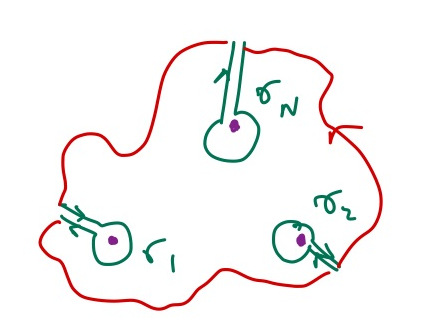
\includegraphics{figs/comp_keyholes}
    \caption{Curve with multiple keyhole cuts.}
  \end{marginfigure}
  \begin{equation}
    \oint_\gamma f(z)\; \mathrm{d}z = \sum_k \oint_{\gamma_k} f(z)\; \mathrm{d}z = 2\pi \zi \sum_{k} \underset{z \to z_k}{\mbox{res}}\ f(z).
  \end{equation}
  \qed
\end{proof}

\begin{example}
  Compute
  \begin{equation*}
    \oint_\gamma \frac{z-1}{(z^2+4)\sin z}\; \mathrm{d}z
  \end{equation*}
  where $z=2\zi$ and $z=0$ lies inside $\gamma$, and $\gamma$ is simple and
  closed.
  
  Noting that $z^2+4 = (z+2\zi)(z-2\zi)$, we have two simple poles inside
  $\gamma$, with residues
  \begin{equation*}
    \underset{z \to 0}{\mbox{res}}\ \frac{1}{\sin z}\frac{z-1}{z^2+4} = \left.\frac{1}{\cos z}\frac{z-1}{z^2+4}\right|_{z=0} = -\frac{1}{4}
  \end{equation*}
  and
  \begin{equation*}
    \underset{z \to 2\zi}{\mbox{res}}\ \frac{z-1}{(z+2\zi)\sin z}\frac{1}{z-2\zi} = \left.\frac{z-1}{(z+2\zi)\sin z}\frac{1}{1!}\right|_{z=2\zi} = \frac{1-2\zi}{4\sinh 2},
  \end{equation*}
  so
  \begin{equation*}
    \oint_\gamma \frac{z-1}{(z^2+4)\sin z}\; \mathrm{d}z = \frac{\pi\zi}{2}\left(\frac{1-2\zi}{\sinh 2} - 1\right).
  \end{equation*}
\end{example}

%-------------------------------------------------------------------------------

\section{Applications for real integrals}

\subsection{Rational functions of $\sin\theta$ and $\cos\theta$}

Sometimes we have real integrals that we wish to evaluate that is actually quite
easy to evaluate if we consider the integral as a complex integral.

\begin{example}
  Find
  \begin{equation*}
    I = \int_0^{2\pi} \frac{\mathrm{d}\theta}{5 - 4 \cos\theta}.
  \end{equation*}
  
  Let $z=\ex^{\zi \theta}$, so $\mathrm{d}z=\zi z\; \mathrm{d}\theta$,
  $\cos\theta = (z+z^{-1})/2$. We have
  \begin{equation*}
    I = \oint_{|z|=1} \frac{1}{\zi z} \frac{\mathrm{d}z}{5 - 4(z+z^{-1})/2} = \oint_{|z|=1}\frac{-1}{\zi} \frac{\mathrm{d}z}{5z - 2z^2 + 2}.
  \end{equation*}
  Noting the denominator factorises to $(2z-1)(z-2)$, the only pole within the
  contour is $z=1/2$, so by Cauchy's integral formula or the residue theorem, we
  have $I = (-2\pi \zi/\zi)(1/2)(-3/2)^{-1} = 2\pi/3$.
\end{example}

\begin{example}
  What about for the above example if the integration domain is instead from $0$
  to $\pi$?
  
  No new calculation really needs to be done here as we can rely on symmetries.
  Note that
  \begin{equation*}
    \int_0^{\pi} \frac{\mathrm{d}\theta}{5 - 4 \cos\theta} = \frac{1}{2}\int_{-\pi}^{\pi} \frac{\mathrm{d}\theta}{5 - 4 \cos\theta}
  \end{equation*}
  since the integrand is an even function about $\theta=0$. However, note also
  that
  \begin{equation*}
    \frac{1}{2}\left(\int^0_{-\pi} + \int^\pi_0\right)\; \mathrm{d}\theta = \frac{1}{2}\left(\int^{2\pi}_\pi + \int^\pi_0\right)\; \mathrm{d}\theta
  \end{equation*}
  by linearity and periodicity, so the relevant integral evaluates to $\pi/3$.
\end{example}

\subsection{Some rational polynomial functions over the real line}

We could also consider some real integrals as segments of the analogous contour
integral extended into complex space. The plan of attack is that we aim to
compute the full contour integral (making use of Cauchy's theorem or the residue
theorem accordingly), and generally aim to show that the segment that is
extended into the complex plane goes to something with increasing distance from the
real line, so the integral we actually wanted on the real line is then the
difference between the full contour integral and the contour integral extended
into the complex plane.\marginnote{If the contour integral extended into the
complex plane is zero as will be for the cases here, then the analogous real
integral is just the full contour integral.}

For this, we note the following two properties:
\begin{proposition}
\begin{itemize}
  \item (estimation) for all $\gamma:[a, b] \to \mathbb{C}$, we have
  \begin{equation}
    \left|\int_\gamma f(z)\; \mathrm{d}z\right| \leq \|\gamma\| \max_\gamma \left|f(\gamma(t))\right|
  \end{equation}
  
  \item (polynomial estimation) a general polynomial is bounded as\marginnote{Can show this by triangle inequality.}
  \begin{equation*}
    \frac{1}{2}\left|a_n z^n\right| \leq \left|a_n z^n + \ldots + a_0 \right| \leq 2\left|a_n z^n\right|.
  \end{equation*}
\end{itemize}
  \qedwhite
\end{proposition}

\begin{example}
  Find
  \begin{equation*}
    I = \int_{-\infty}^\infty \frac{x+3}{(x^2+1)^2}\; \mathrm{d}x.
  \end{equation*}
  
  Here we take $x\to z$ and consider the semi-circle contour $\gamma_R = \ell_R
  + C_R$ as in the figure to the right. The aim is to show that the semi-circle
  part $C_R$ goes to zero as $R\to \infty$.
  
  \begin{marginfigure}
    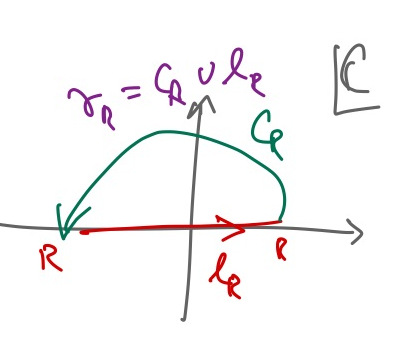
\includegraphics{figs/comp_semicircle_curve}
    \caption{Semi-circle curve with extrusion into the complex plane, with
    $\gamma_R = C_R \cup \ell_R$.}
  \end{marginfigure}
  
  
  For $R > 1$, the residue is at $z=\zi$, and we note that
  \begin{equation*}
    \underset{z \to \zi}{\mbox{res}}\ \frac{z+3}{(z-\zi)^2}\frac{1}{(z+\zi)^2} = \left.\frac{1}{1!} \left(\frac{\mathrm{d}}{\mathrm{d}z} \frac{z+3}{(z+\zi)^2}\right)\right|_{z=\zi} = \frac{3}{4\zi},
  \end{equation*}
  so $\oint f(z)\; \mathrm{d}z = 3\pi/2$ by the residue theorem. Now, we have
  \begin{equation*}
    |(z^2+1)^2| \geq \frac{1}{2}|z|^4, \qquad |z+3| \leq 2|z|,
  \end{equation*}
  so
  \begin{equation*}
    \left|\int_{C_R} f(z)\; \mathrm{d}z\right| \leq \max_{C_R} \left|\frac{z+3}{(z^2+1)^2}\right| \pi R \leq \frac{2R}{R^4/2} \pi R = O\left(\frac{1}{R^2}\right),
  \end{equation*}
  thus the integral goes to zero as $R\to\infty$ by the absolute convergence
  theorem. By linearity of integrals, 
  \begin{equation*}
    \frac{3\pi}{2} = \oint_{\gamma_R} f(z)\; \mathrm{d}z = \left(\int_{\ell_R} + \int_{C_R}\right) f(z)\; \mathrm{d}z \to I,
  \end{equation*}
  so that
  \begin{equation*}
    \int_{-\infty}^\infty \frac{x+3}{(x^2+1)^2}\; \mathrm{d}x = \frac{3\pi}{2}.
  \end{equation*}
\end{example}

\begin{example}
  Find
  \begin{equation*}
    I = \int_{-\infty}^\infty \frac{1}{x^2 - 2x + 5}\; \mathrm{d}x.
  \end{equation*}
  
  The function has a pole at $z_0 = 1+2\zi$ (via the use of the quadratic
  formula for example), with residue $-\zi/4$. Using the semi-circle contour as
  above, we have also
  \begin{equation*}
    \left|\int_{C_R} f(z)\; \mathrm{d}z\right| = O\left(\frac{1}{R}\right),
  \end{equation*}
  so $I = 2\pi\zi(-\zi /4) = \pi/2$.
\end{example}

\begin{example}
  Find
  \begin{equation*}
    I = \int_{-\infty}^\infty \frac{\cos x}{x^2 +1}\; \mathrm{d}x.
  \end{equation*}
  
  We consider instead
  \begin{equation*}
    I' = \mbox{Re}\int_{-\infty}^\infty \frac{\ex^{\zi x}}{x^2 +1}\; \mathrm{d}x.
  \end{equation*}
  On the semi-circle extended into the complex plane, we have
  \begin{equation*}
    \left|\int_{C_R} \frac{\ex^{\zi z}}{z^2+1}\; \mathrm{d}z\right| \leq |\ex^{\zi z}| O\left(\frac{1}{R}\right).
  \end{equation*}
  Since $|\ex^{\zi z}|$ is bounded by unity, the integral on $C_R$ goes to zero
  as $R\to\infty$. On the other hand, the integrand has a simple pole at
  $z=\zi$, where
  \begin{equation*}
    \underset{z \to \zi}{\mbox{res}}\ \frac{1}{z-\zi}\frac{\ex^{\zi z}}{z+\zi} = \left.\frac{\ex^{\zi z}}{z+\zi} \frac{1}{1!}\right|_{z=\zi} = \frac{\zi}{2\ex},
  \end{equation*}
  so $I' = \pi/\ex$, which is purely real. So we have\marginnote{The sine one could have been anticipated since the integrand
  there is odd about $x=0$.}
  \begin{equation*}
    \int_{-\infty}^\infty \frac{\cos x}{x^2 +1}\; \mathrm{d}x = \frac{\pi}{\ex}, \qquad \int_{-\infty}^\infty \frac{\sin x}{x^2 +1}\; \mathrm{d}x = 0.
  \end{equation*}
\end{example}

If there are singularities on the real line itself, then we could in principle
`indent' the contour on the real line to bypass the singularities in the way.

\begin{lemma}[Indentation lemma]
  Let $f$ have a simple pole at $z=a$, then\marginnote{The $\pi\zi$ factor comes
  from going halfway around the full circle, although to show this properly is
  non-trivial. This also only works for simple poles (essentially assumes small
  $R$ and there is a Laurent expansions where terms can be bound accordingly).}
  \begin{equation}
    \lim_{z\to a} \int_{C_R} f(z)\; \mathrm{d}z = \pi\zi\underset{z \to a}{\mbox{res}}\ f(z),
  \end{equation}
  where the pole is assumed to be bypassed in the positive (anti-clockwise)
  sense.
  
  \qedwhite
\end{lemma}

\begin{example}
  Find the integral of the (unnormalised) \textbf{sinc function}
  \begin{equation*}
    I = \int_{-\infty}^\infty \frac{\sin x}{x}\; \mathrm{d}x.
  \end{equation*}
  
  Here what we do is take an indented semi-circle contour as in the figure on
  the right, and compute each parts separately.
  
  Starting with the upper semi-circle arc $C_R$, the standard estimate tells us
  the integral on the semi-circle goes as $O(1)$ even if we bound $\sin x$ by
  unity, so we need to work a bit harder. Note that by doing integral by parts,
  we have
  \begin{marginfigure}
    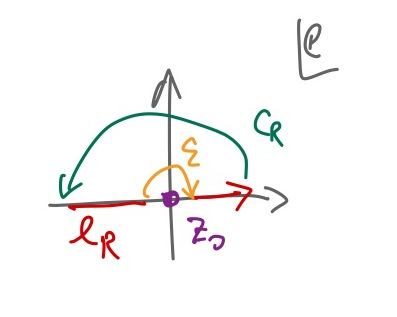
\includegraphics{figs/comp_semicircle_indent}
    \caption{Curve with indentation in the \emph{negative} sense around a pole,
    where $\gamma_R = C_R \cup \ell_R \cup \epsilon$.}
  \end{marginfigure}
  \begin{equation*}
    \int_{C_R} \frac{1}{z}\ex^{\zi z}\; \mathrm{d}z = \left[\frac{1}{z}\frac{\ex^{\zi z}}{\zi}\right]^R_{-R} + \frac{1}{\zi} \int_{C_R} \frac{1}{z^2} \ex^{\zi z}\; \mathrm{d}z.
  \end{equation*}
  Since the exponential terms are bounded by unity, both the boundary as well as
  the integral in this case behaves as $O(1/R^2)$ as $R\to\infty$, so we have
  what we need from the integral extruded into the complex plane.
  
  For the indented part, we note here that $z=0$ is a pole with residue $1$, and
  noting that we are going clockwise \emph{above} the pole thus giving as an
  extra minus sign, the integral is $-\pi \zi$. Now, by Cauchy's theorem, the
  closed integral over the indented semi-circle since there are no singularities
  within the contour, and so we have
  \begin{align*}
    0 = \oint_{\gamma_R} f(z)\; \mathrm{d}z &= \left(\int_\epsilon + \int_{C_R} + \int^R_{-R}\right)f(z)\; \mathrm{d}z \\
      & \to -\pi \zi + 0 + \int^\infty_{-\infty} f(z)\; \mathrm{d}z
  \end{align*}
  as $R\to\infty$. Together, we have
  \begin{equation*}
    I = \mbox{Im} \int_{-\infty}^\infty \frac{\ex^{\zi z}}{z}\; \mathrm{d}z = \mbox{Im} (\pi \zi) = \pi.
  \end{equation*}
\end{example}

%===============================================================================

\chapter{More analysis topics}

This chapter contains a collection of results that utilises some previous
integration techniques.

%-------------------------------------------------------------------------------

\section{Some theorems}

%%%%%%%%%%

\subsection{Liouville's theorem}

\begin{theorem}
  A bounded entire function is constant.
\end{theorem}

\begin{proof}
  Applying Cauchy's integral formula, we get
  \begin{equation*}
    f(a) - f(b) = \frac{1}{2\pi\zi}\oint_\gamma\left( \frac{f(z)}{z-a} - \frac{f(z)}{z-b}\right)\; \mathrm{d}z,
  \end{equation*}
  with $\gamma$ chosen such that $\gamma$ is a circle of radius $R$ centred on
  $b$, with $R$ large enough to contain $a$. We see then
  \begin{equation*}
    f(a) - f(b) = \frac{a-b}{2\pi\zi}\oint_\gamma \frac{f(z)}{(z-a)(z-b)}\; \mathrm{d}z.
  \end{equation*}
  Since $z\in\gamma$, we note that $|z-b| = R$, while
  \begin{equation*}
    |z-a| = |z - b + b -a| \geq |z-b| - |b-a| \geq \frac{R}{2}.
  \end{equation*}
  Thus we have (since $f(z) \leq K$ is assumed to be bounded)
  \begin{align*}
    |f(a) - f(b)| &= \left|\frac{b-a}{2\pi\zi}\right| \cdot \left| \oint_\gamma \frac{f(z)}{(z-a)(z-b)}\; \mathrm{d}z\right|\\
      &\leq \frac{|b-a|}{2\pi} \oint_\gamma \frac{K}{R \cdot R/2}\; |\mathrm{d}z| \\
      &= \frac{|b-a|}{2\pi} \frac{2K}{R^2} 2\pi R \\
      &\to 0
  \end{align*}
  as $R\to\infty$, hence $f(a) = f(b)$, i.e. a constant entire function. \qed
\end{proof}

%%%%%%%%%%

\subsection{Cauchy's inequality}

\begin{lemma}
  Let $f:D(a;r) \subset \mathbb{C} \to \mathbb{C}$ be holomorphic, then
  \begin{equation}
    \left|f^{(n)}(a)\right| \leq K\frac{n!}{r^n},
  \end{equation}
  where $D(a; r) = \{z\in\mathbb{C}\ |\ |z-a| < r\}$ is the disk centred at
  $z=a$ of radius $r$, for $n=0, 1, \ldots$, and such that $|f(z)| \leq K$ for
  $z\in D(a;r)$.
\end{lemma}

\begin{proof}
  By Cauchy's integral formula, we have
  \begin{equation*}
    f^{(n)}(a) = \frac{n!}{2\pi\zi} \oint_{\partial D(a;r)} \frac{f(z)}{(z-a)^{n+1}}\; \mathrm{d}z,
  \end{equation*}
  so that
  \begin{equation*}
    \left|f^{(n)}(a)\right| \leq \frac{n!}{2\pi} \frac{K}{r^{n+1}} 2\pi r = K\frac{n!}{r^n}.
  \end{equation*}
  \qed
\end{proof}

\begin{corollary}
  Applying Cauchy's inequality to some $a\in\mathbb{C}$ we see that $|f'(a)| \to
  0$ as $R\to\infty$, showing that $f$ is an entire constant function, and
  provides a simpler proof to Liouville's theorem.
\end{corollary}

%%%%%%%%%%

\subsection{Fundamental theorem of algebra}

\begin{theorem}
  A polynomial of degree $n\geq1$ has $n$ roots in $\mathbb{C}$ if the leading
  coefficient is non-zero.
\end{theorem}

\begin{proof}
  We suppose otherwise, and that the polynomial $p(z)$ has no roots at all in
  $\mathbb{C}$. So then since $p(z) \neq 0$, $p^{-1}(z)$ is holomorphic on
  $\mathbb{C}$. The leading coefficient of $p(z)$ is non-zero, so $f(z) =
  p^{-1}(z)$ is not constant. So, by triangle inequality,
  \begin{equation*}
    |p(z)| \geq |a_n| |z|^n - |a_0| - |a_1||z| - \ldots |a_{n-1}||z|^{n-1}.
  \end{equation*}
  Let
  \begin{equation*}
    a = \sum_{i=0}^{n-1} |a_i|,
  \end{equation*}
  then for $|z| > 1$, we have
  \begin{equation*}
    |p(z)| \geq |z|^{n-1} \left(|a_n||z| - \frac{|a_0|}{|z|^{n-1}} - \ldots \frac{|a_{-1}|}{1}\right) \geq |z|^{n-1}\left(|a_n||z| - a\right).
  \end{equation*}
  Let $K = \max\{1, (M+a)/|a_n|\}$. We see that if $|z| > K$ then $|p(z)| > M$,
  and hence $|p(z)|^{-1} < M^{-1}$. 
  
  But for $|z| \leq K$, $f(z) = p^{-1}(z)$ is bounded in the absolute value
  because it is holomorphic, hence it is continuous. If this bound is $L$, then
  for all $z$, $|f(z)| < \max\{M^{-1}, L\}$ and hence we have a bounded entire
  function, which is a contradiction according to Liouville's theorem. Thus
  $p(z)$ has a root in $\mathbb{C}$, and we factorise the root out and continue
  by induction until the remaining polynomial has zero degree, i.e. a constant. \qed
\end{proof}

%%%%%%%%%%

\subsection{Maximum principle}

\begin{theorem}[Maximum modulus principle]
  Let $f: U \subset \mathbb{C} \to \mathbb{C}$ be holomorphic with $\partial U$
  a simple closed curve. Assuming $f$ is non-constant and that $|f(z_0)| =
  \max_{z\in\overline{U}}|f(z)|$, then $z_0 \in \partial U$, i.e. occurs on the
  boundary. \qedwhite
\end{theorem}

\begin{example}
  Find all $f: D(0,1) \to \mathbb{C}$ that are holomorphic and satisfy $f(0) =
  1$, $|f| \geq 1$ for all $z \in D(0, 1)$.
  
  The inequality is the wrong way round so we consider $g = 1/f$. Note that
  $g(0) = 1$, $g$ is holomorphic, and $|g| \leq 1$ in the unit disk by
  construction. Then assuming $g$ is non-constant, by the maximum principle we
  have
  \begin{equation*}
    1 = |g(0)| < \max_{\partial D} |f| \leq \max_D |f| = 1,
  \end{equation*}
  which gives a contradiction, so $g$ and thus $f$ is a constant, which in this
  case means $f(z) \equiv 1$.
\end{example}

\begin{example}
  Find the maximum value of $|f(z)|$ in the unit disk for $f(z) = z^2 - 3z + 2$.
  
  $f$ is holomorphic on the unit disk and the boundary is simple and closed, so
  by the maximum principle, for $z \in \overline{D(0, 1)}$,
  \begin{align*}
    |f(z)| \leq \max_{|w|\leq 1} |f(w)| &= \max_{\theta \in [0, 2\pi]}\left|f(\ex^{\zi\theta})\right|\\
      & \max_{\theta \in [0, 2\pi]} \sqrt{(\ex^{2\zi\theta}-3\ex^{\zi\theta} + 2)\ex^{-2\zi\theta}-3\ex^{-\zi\theta} + 2)}\\
      & = \max_{\theta \in [0, 2\pi]} \sqrt{14 - 18 \cos\theta + 4\cos 2\theta}.
  \end{align*}
  The extrema are at $\theta = 0, \pi$, and the latter turns out to be the
  maximiser, and $|f(z)| \leq 6$.
\end{example}

%%%%%%%%%%

\subsection{Argument theorem}

\begin{theorem}[Argument theorem]
  Let $f: U \subset \mathbb{C} \to \mathbb{C}$ be holomorphic on $U \ \{w_1,
  \ldots w_\ell\}$ and poles of order $p_i\in\mathbb{N}$ at $w_j$, and assume
  that $\partial U$ is a simple closed curve.\marginnote{e.g. keyhole indented
  curves.} Let $z_1, \ldots z_m \in U$ be the zeroes of $f$ with order $n_j$. If
  \begin{equation*}
    \sum_1^{\ell} p_j = P, \quad \sum_1^m n_j = N,
  \end{equation*}
  then
  \begin{equation}
    \frac{1}{2\pi\zi} \oint_{\partial U} \frac{f'}{f}\; \mathrm{d}z = N - P.
  \end{equation}
\end{theorem}

\begin{proof}
  We see that
  \begin{equation*}
    \frac{1}{2\pi\zi}\oint_{\gamma_j} \frac{f'}{f}\; \mathrm{d}z = -p_j, \quad 
    \frac{1}{2\pi\zi}\oint_{\Gamma_j} \frac{f'}{f}\; \mathrm{d}z =  n_j,
  \end{equation*}
  where $\gamma_j$ are the indented curves circling the poles and $\Gamma_j$ are
  the indented curves circling the zeroes\marginnote{Both following on from
  residue theorem.}transversing in the negative sense. Then, constructing the
  curve that is the union of $\partial U$, $\Gamma_j$ and $\gamma_j$ such that
  $f'/f$ contain no zeros or poles, we have by Cauchy's theorem (and
  transversing the indented curves in the negative sense)
  \begin{align*}
    0 &= \frac{1}{2\pi\zi} \oint_{\partial U} \frac{f'}{f}\; \mathrm{d}z + \frac{1}{2\pi\zi}\oint_{\gamma_j} \frac{f'}{f} + \frac{1}{2\pi\zi}\oint_{\Gamma_j} \frac{f'}{f}\; \mathrm{d}z \\
      &= \frac{1}{2\pi\zi} \oint_{\partial U} \frac{f'}{f}\; \mathrm{d}z + \sum_1^m (-n_j) + \sum_1^\ell p_j,
  \end{align*}
  from which the result follows. \qed
\end{proof}

\begin{example}
  Let $f = z^5 - 3\zi z^3 + z - 20$ and let $\gamma$ be a curve which encloses
  all zeroes of $f$. Evaluate
  \begin{equation*}
    I = \oint_\gamma \frac{5z^4 - 2\zi z^2 + 1}{z^5 - 3\zi z^3 + z - 20}\; \mathrm{d}z.
  \end{equation*}
  
  By the argument theorem, note that $f$ has five zeroes and no poles, so $I =
  2\pi\zi(5-0) = 10\pi zi$.
\end{example}

Following on from the argument theorem, the local version is as follows. Let $f:
U \subset \mathbb{C} \to \mathbb{C}$ be holomorphic and let $f$ have a zero of
order $n\ \geq 1$ at $a \in U$. Taylor's theorem says that
\begin{equation*}
  f(z) = \sum_{k=n}^\infty a_k (z-a)^k = (z-a)^n \sum_{k=n}^\infty a_k (z-a)^{k-n} = (z-a)^n g(z),
\end{equation*}
where $g(z)$ is holomorphic and $g(a) = a_n \neq 0$ by assumption. We see that
we have
\begin{equation*}
  \frac{f'}{f} = \frac{\mathrm{d}}{\mathrm{d}z}\log f(z) = \frac{\mathrm{d}}{\mathrm{d}z} \log (z-a)^n + \frac{\mathrm{d}}{\mathrm{d}z} \log g(z) = \frac{n}{z-a} + \frac{g'}{g}.
\end{equation*}
Since $g(a) \neq 0$, we have $g$ holomorphic in some $D(a, r)$ for small $r$. So
then
\begin{equation*}
  \frac{1}{2\pi\zi} \oint_{\partial D} \frac{f'}{f}\; \mathrm{d}z = \frac{1}{2\pi\zi} \oint_{\partial D} \left(\frac{n}{z-a} + \frac{g'}{g}\right)\; \mathrm{d}z = n
\end{equation*}
by Residue theorem and Cauchy's theorem. Hence if $f$ has a zero of order $n$ at
$z=a$, then
\begin{equation}
  \oint_{\partial D} \frac{f'}{f}\; \mathrm{d}z = 2\pi\zi n.
\end{equation}

By a similar argument, if $f$ has a pole of order $p \geq 1$ at $z=b$, then the
Laurent series will be
\begin{equation*}
  f(z) = \sum_{k=-p}^\infty a_k (z-b)^k = (z-b)^{-p} \sum_{k=-p}^\infty a_k (z+p)^{k-n} = (z-b)^{-p} g(z),
\end{equation*}
with $a_{-p} \neq 0$, so that
\begin{equation}
  \oint_{\partial D} \frac{f'}{f}\; \mathrm{d}z = -2\pi\zi p.
\end{equation}

%%%%%%%%%%

\subsection{Rouche's theorem}

\begin{theorem}
  Let $f, g: U \subset \mathbb{C} \to \mathbb{C}$ be holomorphic and $\partial
  U$ be simple and closed. If $|g| < |f|$ on $\partial U$, then $f(z)$ and $f(z)
  + g(z)$ have the same number of solutions in $U$.\marginnote{From Wikipedia:
  if a person were to walk a dog on a leash around and around a tree, such that
  the distance between the person and the tree is always greater than the length
  of the leash, then the person and the dog go around the tree the same number
  of times.}
\end{theorem}

\begin{proof}
  Consider $F(z) = g(z) / f(z)$, and let $N_1$ and $N_2$ be the number of zeroes
  of $f+g$ and $f$ in $U$ respectively. By the argument theorem, we have
  \begin{equation*}
    N_1 = \oint_{\partial U} \frac{f'+g'}{f+g}\; \mathrm{d}z, \quad 
    N_2 = \oint_{\partial U} \frac{f'}{f}\; \mathrm{d}z,
  \end{equation*}
  and there are no poles since the functions are holomorphic. We note, then
  \begin{align*}
    N_1 - N_2 &= \frac{1}{2\pi\zi} \left[\oint_{\partial U} \frac{f'+g'F + fF'}{f+fF}\; \mathrm{d}z - \oint_{\partial U} \frac{f'}{f}\; \mathrm{d}z\right]\\
      &=\frac{1}{2\pi\zi}\oint_{\partial U} \frac{F'}{f(1+F)}\; \mathrm{d}z.
  \end{align*}
  Since $|F| = |g/f| < 1$ by assumption, we can Taylor expand and obtain
  \begin{equation*}
    N_1 - N_2 = \frac{1}{2\pi\zi}\oint_{\partial U} F' (1 - F + F^2 + \ldots)\; \mathrm{d}z.
  \end{equation*}
  Notice however that $F'F^k \sim (F^{k+1})'$ for sensible values of integer
  $k$, so by fundamental theorem of calculus, we conclude that the integral is
  zero, so that $N_1 = N_2$.
  \qed
\end{proof}

\begin{proof}[Alternate proof of the Fundamental Theorem of Algebra]
  We can actually use Rouche's theorem. Let $f = a_n z^n$ and $g = \sum_i^{n-1}
  a_i z^i$, and make use of the fact that $f$ has $n$ zeroes in the domain (the
  roots of unity). Then on $|z| = r > 1$, we have
  \begin{equation*}
    \left|\frac{g}{z}\right| = \frac{|\sum a_i z^i|}{|a_n z^n|} \leq \frac{\sum_i |a_i|r^i}{|a_n| r^n} \leq \frac{\sum_i |a_i|r^{n-1}}{|a_n| r^n}
  \end{equation*}
  since $r > 1$. So since $|g/f| \to 0$ as $r\to \infty$, we can invoke Rouche's
  theorem, so that $f + g = \sum_i^n a_i z^i$ has the same amount of zeroes as
  $f = a_n z^n$ within $\mathbb{C}$. \qed
\end{proof}

\begin{example}
  Show that all roots of $z^7 - 5z^3 + 12 = 0$ lie in the annulus $1 \leq |z| <
  2$.
  
  We aim to show there are no roots in the unit circle and seven roots in the
  circle of radius two, so by fundamental theorem of calculus we account for all
  the roots within the annulus. Let $f = 12$ and $g = ^7 - 5z^3$ on $|z| < 1$.
  For this choice we have
  \begin{equation*}
    |f| = 12, \quad |g| = |z^7 + 5z^3| < |z|^7 + 5|z|^3 = 6,
  \end{equation*}
  so $|f| > |g|$, and since $f$ has no roots in the unit circle, neither does
  $f+g$.
  
  Within the circle of radius two, we let $f = z^7$ and $g = 12 - 5z^3$. Then
  \begin{equation*}
    |f| = 128, \quad |g| = |12 - 5z^3| < 12 + 5|z|^3 = 52,
  \end{equation*}
  so $|f| > |g|$, and since $f$ has seven roots here, so does $f+g$. By
  fundamental theorem of algebra, $f+g$ can only have seven roots, so all roots
  occur in the target annulus.
\end{example}

%%%%%%%%%%

\subsection{Zeroes of holomorphic functions}

Let $A\subset \mathbb{C}$ and $a\in A$, then $a$ is \textbf{isolated} in $A$ if
there exists some $\epsilon > 0$ such that the intersection of the disk $D(a,
\epsilon)$ with $A$ is simply the point $a$.

\begin{theorem}
  Let $f: U \subset \mathbb{C} \to \mathbb{C}$ be holomorphic and denoting
  $Z(f)$ to be the set of $z\in U$ that are zeroes of $f$. Assuming $f(z)$ is
  not identically zero, then $Z(f)$ is discrete.\marginnote{Or, there are no
  `lines' or `areas' of zeroes for non-trivial functions.} \qedwhite
\end{theorem}

\begin{theorem}[Uniqueness theorem]
   Let $f: U \subset \mathbb{C} \to \mathbb{C}$ be holomorphic and $U$ is
   connected. If $Z(f)$ is not discrete, then $f(z) \equiv 0$. \qedwhite
\end{theorem}

\begin{example}
  Find all holomorphic functions $f:D(0, 1) \to \mathbb{C}$ where $f(1/n) = 1/n$
  for $n\in\mathbb{N}$.
  
  Consider the holomorphic function $g(z) = f(z) - z$, then clearly $\{0, 1/n\}
  \subseteq Z(g)$ by construction. However, $z=0$ is no isolated since $1/n\to
  0$ for $n\to \infty$, so $g(z) \equiv 0$, and so $f(z) = z$ is the only
  choice.
\end{example}

%-------------------------------------------------------------------------------

\section{Pointwise and uniform convergence}

\begin{theorem}[Weierstrauss $M$-test]

\qed

\end{theorem}

\begin{theorem}

\qed

\end{theorem}

\begin{theorem}

\qed

\end{theorem}

%===============================================================================

\chapter{Conformal mapping}

A mapping $f: A \to B$ is called \textbf{conformal} if for each $z_0 \in A$, $f$
rotates tangent vectors of curves through $z_0$ by a definite angle $\theta$ and
a stretch factor $r$. A conformal map preserves angles.

\begin{example}
  We have a few simple examples of conform maps:
  \begin{itemize}
    \item \emph{translations} $f(z) = z+\alpha$, $\alpha \in \mathbb{C}$
    \item \emph{rotations} $f(z) = \ex^{\zi \theta}$, $\theta \in \mathbb{R}$
    \item \emph{stretching} $f(z) = \beta z$, $\beta \in \mathbb{R}^+$
    \item \emph{inversion} $f(z) = 1/z$
  \end{itemize}
\end{example}

\begin{theorem}
  Let $f: U \to \mathbb{C}$ be holomorphic, then $f$ is conformal if and only if
  and $f'(z) \neq 0$ for all $z\in U$.
\end{theorem}

\begin{proof}
  We see that, by definition, for any curve $\gamma(t) \in U$ with $\gamma(0) =
  z_0$ where $\gamma'(0) \neq 0$, the transformed curve $\sigma(t) =
  f(\gamma(t))$ is differentiable at $t=0$. Let $u = \sigma'(0)$ and $v =
  \gamma'(0)$, we have, assuming $f$ is conformal,
  \begin{equation*}
    |u| = r|v|, \qquad \mathrm{arg} v + \theta\ (\mathrm{mod}\ 2\pi) = \mathrm{arg} u.
  \end{equation*}
  By chain rule, $u = \sigma'(0) = f'(z_0) \gamma'(0) = f'(z_0) v$, which
  implies
  \begin{equation*}
    r = |f'(z_0)|, \qquad \theta = \mathrm{arg}\ f'(z_0),
  \end{equation*}
  which for non-zero curves is only true if $f'(z_0) \neq 0$. \qed
\end{proof}

The aforementioned maps are conformal (with special circumstances for the
inversion map).

\begin{theorem}[Inverse function theorem]
  Let $f: U \to \mathbb{C}$ be conformal and $\partial U$ be simple and closed.
  $f$ by definition is invertible, and $f^{-1} : \mathrm{Im}(f) \to U$ is such
  that $f^{-1}$ is also conformal. \qedwhite
\end{theorem}

\begin{theorem}
  All conformal maps preserve the angles of two curves at their respective
  intersections.
\end{theorem}

%%%%%%%%%%

\subsection{M\"obius transformations}

A \textbf{M\"obius transformation} is a map of the form
\begin{equation}
  T(z) = \frac{az + b}{cz + d}
\end{equation}
where $a,b,c,d \in \mathbb{C}$ and $ad - bc \neq 0$.\marginnote{Note $ad-bc$ looking like the determinant of a $2\times2$ matrix is not a coincidence.}

\begin{theorem}
  We have the following properties for M\"obius maps:
  \begin{itemize}
    \item $T(z)$ is holomorphic for $z \neq -d/c$
    \item $T'(z)$ is not zero for $z \neq -d/c$ \marginnote{So M\"obius maps are
    conformal except at $z = d/c$.}
    \item for every $T(z)$ there exists an inverse $T^{-1}(z)$ that is also a
    M\"obius map\marginnote{Related to a non-vanishing determinant.}
    \item the \textbf{cross ratios}
    \begin{equation}
      [z_1, z_2 : z_3, z_4] = \frac{(z_1 - z_3)(z_2 - z_4)}{(z_1 - z_4)(z_2 - z_3)}
    \end{equation}
    are invariant under M\"obius transformations, i.e.
    \begin{equation*}
      [z_1, z_2 : z_3, z_4] = [T(z_1), T(z_2) : T(z_3), T(z_4)]
    \end{equation*}
  \end{itemize}
  \qedwhite
\end{theorem}

\begin{theorem}

\qedwhite

\end{theorem}

%-------------------------------------------------------------------------------

\section{Harmonic functions}

\begin{theorem}

\qed

\end{theorem}

%%%%%%%%%%

\subsection{Dirichlet and Neumann problems}

%%%%%%%%%%

\subsection{Joukowsky transform and aerofoil theory}

%===============================================================================

%%%%%%%%%%%%%%%%%%%%%%%%%%%%%%%%%%%%%%%%%

% r.5 contents
%\tableofcontents

%\listoffigures

%\listoftables

% r.7 dedication
%\cleardoublepage
%~\vfill
%\begin{doublespace}
%\noindent\fontsize{18}{22}\selectfont\itshape
%\nohyphenation
%Dedicated to those who appreciate \LaTeX{} 
%and the work of \mbox{Edward R.~Tufte} 
%and \mbox{Donald E.~Knuth}.
%\end{doublespace}
%\vfill

% r.9 introduction
% \cleardoublepage

%%%%%%%%%%%%%%%%%%%%%%%%%%%%%%%%%%%%%%%%%
% actual useful crap (normal chapters)
\mainmatter

%\part{Basics (?)}


%\backmatter

%\bibliography{refs}
\bibliographystyle{plainnat}

%\printindex

\end{document}

